%!TEX root = ../thesis.tex
%*******************************************************************************
%****************************** Third Chapter **********************************
%*******************************************************************************
\chapter{Generative modelling / autoencoders}

% **************************** Define Graphics Path **************************
\ifpdf
    \graphicspath{{Chapter5/Figs/Raster/}{Chapter5/Figs/PDF/}{Chapter5/Figs/}}
\else
    \graphicspath{{Chapter5/Figs/Vector/}{Chapter5/Figs/}}
\fi

This chapter is based on the paper \emph{On the Latent Space of Wasserstein Auto-Encoders}. This work was published as two separate workshop papers at ICLR 2018.






%\title{On the Latent Space of Wasserstein Auto-Encoders}

% The \author macro works with any number of authors. There are two
% commands used to separate the names and addresses of multiple
% authors: \And and \AND.
%
% Using \And between authors leaves it to LaTeX to determine where to
% break the lines. Using \AND forces a line break at that point. So,
% if LaTeX puts 3 of 4 authors names on the first line, and the last
% on the second line, try using \AND instead of \And before the third
% author name.


%\begin{abstract}
%We study the role of latent space dimensionality in Wasserstein auto-encoders (WAEs). 
%Through experimentation on synthetic and real datasets, we argue that probabilistic encoders should be preferred over deterministic encoders.
%We find that it is non-trivial to train probabilistic-encoder WAEs as training with the original WAE-MMD objective fails in this setting.
%We propose an additional regulariser to resolve this problem, and finally highlight the potential of WAEs for representation learning with promising results on a benchmark disentanglement task.
%\end{abstract}

\section{Introduction}
Unsupervised generative modeling is increasingly attracting the attention of the machine learning community.
Given a collection of unlabelled data points $S_X$, the ultimate goal of the task is to learn a model capable of generating sets of synthetic points $S_G$ which \emph{look similar to} $S_X$.
The closely related field of unsupervised representation learning in addition aims to produce semantically meaningful representations (or features) of the data points~$S_X$.
There are various ways of defining the notion of \emph{similarity} between two sets of data points.
The most common approach assumes that both $S_X$ and $S_G$ are sampled independently from two probability distributions $P_X$ and $P_G$ respectively, and employ some of the known divergence measures for distributions.

Two major approaches currently dominate this field.
Variational Auto-Encoders (VAEs) \citep{KW14, rezende2014stochastic} minimize the Kullback-Leibler (KL) divergence $D_{\KL}(P_X, P_G)$, which is equivalent to maximizing the \emph{marginal log-likelihood} of the model $P_G$.
Generative Adversarial Networks (GANs) \citep{goodfellow2014generative} employ a framework, commonly referred to as \emph{adversarial training}, which is suitable for many different divergence measures, including (but not limited to) $f$-divergences \citep{nowozin2016f}, 1-Wasserstein distance \citep{AB17}, and Maximum Mean Discrepancy (MMD) \citep{dziugaite2015training, li2017mmd, BS+18}.

Both approaches have their pros and cons. 
VAEs can both generate and \emph{encode} (featurize) data points, are stable to train, and typically manage to cover all modes of the data distribution.
Unfortunately, they often produce examples~that are far from the true data manifold.
This is especially true for structured high-dimensional datasets such as natural images, where VAEs generate \emph{blurry}~images.
GANs, on the other hand, are good at producing realistic looking examples (landing on or very close to the manifold), however they cannot featurize the points, often cover only few modes of the data distribution, and are highly unstable to train \citep{salimans2016improved}.

A number of recent papers modify the VAE framework with the goal of improving sample quality. Approaches include using more flexible approximate posteriors \citep{kingma2016improved}, priors \citep{tomczak2017vae} and different ways of blending with adversarial training in the hope of combining the strengths of GANs and VAEs \citep{larsen2015autoencoding, MSJ+16, MNG17}.

Taking a different approach by switching focus from the KL objective to the optimal transport distance, \cite{TBG+17} introduce the Wasserstein Auto-Encoder. This architecture shares many of the desirable properties of VAEs while providing samples of better quality. 
Importantly, WAEs still allow for adversary-free versions, resulting in a min-min training objective leading to stable training.
In this work we aim at further improving the quality of generative modeling and representation learning techniques, focussing on the adversary-free WAE-MMD architecture as we find the instability of the adversarial training to be an unfortunate obstacle when it comes to controlled reproducible experiments.
Our main contributions are threefold.

\textbf{First}, we demonstrate that a mismatch between the latent space dimensionality $\dZ$ and the intrinsic data dimensionality $\dP$ may harm the performance of WAEs when using deterministic encoders as considered in all experiments of \cite{TBG+17}.
For auto-encoder architectures, the quality of generated samples can be no better than that of reconstructed images. Therefore we are interested in training WAEs with larger latent bottlenecks as reconstruction error generally improves with increased latent dimension.
However, we show that generated sample quality actually \emph{degrades} beyond some ideal latent dimension due to the difficulty of distribution matching in higher dimensions.  

\textbf{Second}, we argue that WAEs can be made adaptive to the unknown $\dP$ by using \emph{probabilistic} encoders.
Somewhat unexpectedly, the use of probabilistic encoders with WAEs is not trivial, as we empirically found that in high latent dimensions the variances of the encoding distributions tend to zero, effectively collapsing to deterministic encoders.
We overcome this problem by introducing an additional regulariser; 
however, how to best train probabilistic-encoder WAEs remains an open question that we would encourage interested researchers to pursue.


\textbf{Third}, we evaluate the usefulness of probabilistic-encoder WAEs for representation learning using the \emph{dSprites} dataset \citep{dsprites17}, a benchmark task in learning \emph{disentangled representations}. We evaluate our method using metrics introduced by three recent papers \citep{HM+17, kumar2017variational, kim2018disentangling}, finding that our method achieves competitive performance on this task compared to state-of-the-art methods introduced by the aforementioned papers.

%We finish this section with a short description of WAEs, preliminaries, and notations.
\subsection*{Short introduction to Wasserstein auto-encoders}

Similarly to VAEs, WAEs describe a particular way to train probabilistic \emph{latent variable models} (LVMs) $P_G$.
LVMs act by first sampling a code (feature) vector $Z$ from a \emph{prior distribution} $P_Z$ defined over the latent space $\Z$ and then mapping it to a random input point $X\in\X$ using a conditional distribution $P_G(X|Z)$ also known as \emph{the decoder} or \emph{generator}.
We will be mostly working with image datasets, so for simplicity we set $\X=\R^{\dX}$,\:$\Z=\R^{\dZ}$, and refer to points $x\in\X$ as pictures, images, or inputs interchangeably.

Instead of minimizing the KL divergence between the LVM $P_G$ and the unknown data distribution $P_X$ as done by VAEs, WAEs aim at minimizing the optimal transport distance between them.
Given any non-negative cost function $c(x,x')$ between two images, WAEs minimize the following objective
with respect to parameters of the \emph{deterministic} decoder ${P_G(X|Z=z)}=\delta_{G(z)}$ mapping\footnote{Here $\delta_t$ is a point distribution supported on $t$.} codes $z\in \Z$ to pictures $G(z)\in \X$:
%\vspace{-.3cm}
\begin{equation}
\label{eq:WAEobj}
\min_{Q(Z|X)}\; \mathop{\E}\limits_{P_X}\; \mathop{\E}\limits_{Q(Z|X)}\bigl[ c\bigl(X, G(Z)\bigr) \bigr] + \lambda \cdot\mathcal{D}_Z(Q_Z, P_Z),
\end{equation}
where the conditional distributions $Q(Z|X)$ are commonly known as \emph{encoders}, 
$Q_Z(Z):= \int Q(Z|X) P_X(X) dX$ is \emph{the aggregated posterior} distribution,
$\mathcal{D}_Z$ is any divergence measure between two distributions over $\Z$, and
$\lambda>0$ is a regularization coefficient.
In practice $Q(Z|X=x)$ and $G(z)$ are often parametrized with deep nets, in which case back propagation can be used with stochastic gradient descent techniques to optimize the objective.

An important design choice that must be made when using a WAE is whether the encoder should map an image $x\in\mathcal{X}$ to a \emph{distribution} $Q(Z|X=x)$ over the latent space or to a single code $z = \varphi(x)\in\mathcal{Z}$,~i.e.\:$Q(Z|X=x) = \delta_{\varphi(x)}$. We refer to the former type as \emph{probabilistic} encoders and the latter as \emph{deterministic} encoders. In practice, the reparametrisation trick, commonly employed in the training of VAEs, may be used in the case of probabilistic encoders.

The objective \eqref{eq:WAEobj} is similar to that of the VAE and has two terms. 
The first \emph{reconstruction term} aligns the encoder-decoder pair so that the encoded images can be accurately reconstructed by the decoder as measured by the cost function $c$ (we will only use the \emph{cross-entropy loss}  throughout).

The second regularization term is different from VAEs: it forces the aggregated posterior $Q_Z$ to match the prior distribution $P_Z$ rather than asking point-wise posteriors $Q(Z|X=x)$ to match $P_Z$ simultaneously for all data points~$x$.
To better understand the difference, note that $Q_Z$ is the distribution obtained by averaging conditional distributions $Q(Z|X=x)$ for all different points $x$ drawn from the data distribution $P_X$.
This means that WAEs explicitly control the shape of the \emph{entire} encoded dataset while VAEs constrain every input point separately.

Both existing versions of the algorithm---WAE-GAN based on adversarial training and the adversary-free WAE-MMD based on the maximum mean discrepancy, only the latter of which we use in this paper---allow for \emph{any} prior distributions $P_Z$ and encoders $Q(Z|X)$ as long as $P_Z$ and $Q_Z$ can be efficiently sampled.
As a result, the WAE model may be easily endowed  with prior knowledge about the possible structure of the dataset through the choice of $P_Z$.

\emph{Notation.} We denote $\varphi(x) = \mathbb{E}\left[Q(Z|X=x)\right]$ to be the mean of the encoding distribution for a given input $x$. By $\varphi_i(x)$ we mean the $i$th coordinate of $\varphi(x)$, $1\leq i \leq \dZ$, and by $P_Z(Z_i)$ and $Q_Z(Z_i)$ the marginal distributions of the prior and aggregated posteriors over the $i$th dimension of $\Z$ respectively. 

\emph{A note on implementation and code.} Throughout, we train all WAE models using Algorithm 2 (WAE-MMD) of \cite{TBG+17} optionally with an additional regulariser that we introduce in Section \ref{section:L1_reg}. Experimental details not present in the main text may be found in the Supplementary Materials. All code for all experiments will be made public upon successful publication. 


\section{Dimension mismatch and probabilistic encoders\label{section:fading-squares}}

What happens if a deterministic-encoder WAE is trained with a latent space of dimension $\dZ$ that is larger than the intrinsic dimensionality $\dI$\footnote{
	$\dI$ is informally the minimum number of parameters required to continuously parametrise the data manifold.
	%It may be possible that $P_Z$ is supported on a low-dimensional subspace of $\Z$, e.g.\:on a hypersphere. 
	%However, this is irrelevant for the priors we consider in this work, which are either Gaussian or uniform on $[-1,1]^{\dZ}$ and thus the intrinsic dimensionality of $P_Z$ is $\dZ$.
} of the data distribution? If the encoder is continuous then the data distribution $P_X$ will be mapped to $Q_Z$ supported on a latent manifold of dimension at most $\dI < \dZ$ while the regularizer in \eqref{eq:WAEobj} will encourage the encoder to fill the latent space similarly to the prior $P_Z$ as much as possible.
This is a hard task for the encoder for the same reason that it is hard to fill the plane with a one dimensional curve.

To empirically investigate this setting, we introduce the simple synthetic \emph{fading squares} dataset consisting of $32 \times 32$ pixel images of centred, $6\times 6$ pixel grey squares on a black background. The value of this colour varies uniformly from $0$ (black) to $1$ (white) in steps of $10^{-3}$. The intrinsic dimensionality of this dataset is therefore $1$, as each image in the dataset can be uniquely identified by the value of the colour of its grey square. 

We trained a deterministic-encoder WAE with a uniform prior over $[-1, 1]^2$.
Since $\dZ=2$, we can easily visualise the learned embedding of the data into the latent space and the output of the decoder across the whole latent space. This is displayed in Figure \ref{fig:fading-squares-latent} (left two plots) for one such WAE.

The WAE is forced to reconstruct the images well, while at the same time trying to fill the latent space uniformly with the 1-dimensional data manifold. The only way to do this is by curling up the data-manifold in the latent space. In practice, the WAE must only fill the space to the extent that it fools the divergence measure which sees only a mini-batch of samples at each training step.
We found that larger mini-batches resulted in tighter curling of the manifold supporting $Q_Z$, suggesting that mini-batch size may strongly affect the performance of WAEs via estimation of $D(Q_Z, P_Z)$.

\begin{figure*}[t]
	\centering
	\begin{minipage}{.25\textwidth}
		\centering
		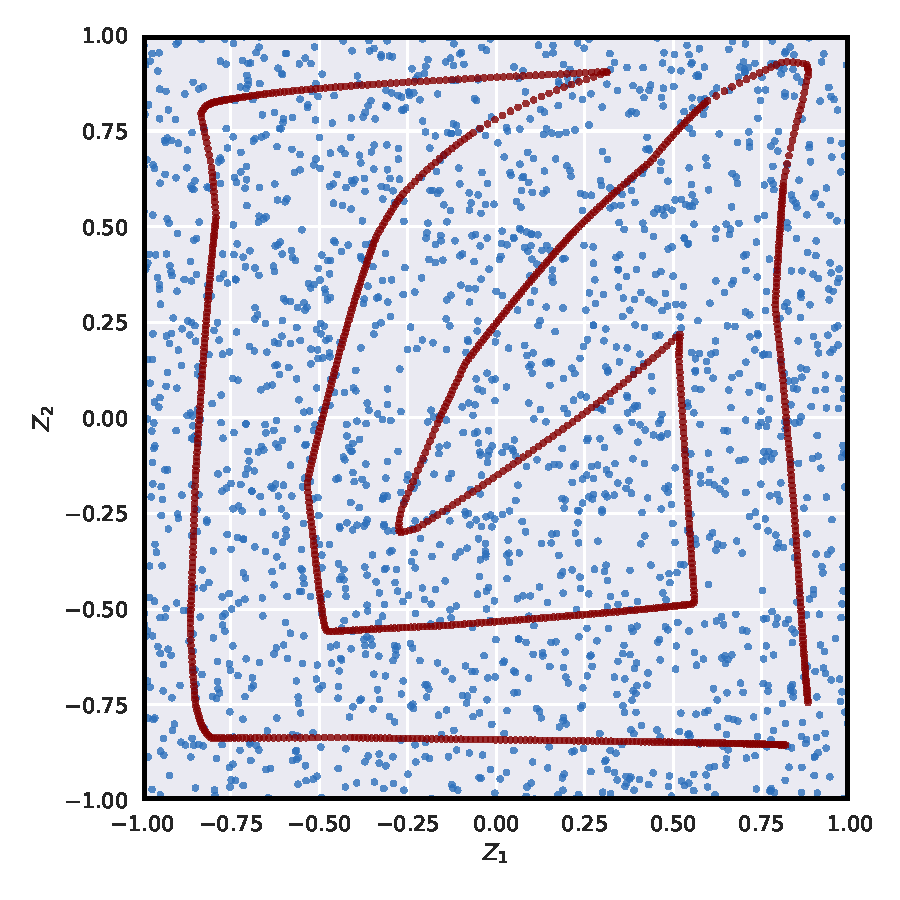
\includegraphics[width=\textwidth]{figures/deterministic_manifold_all}

		
	\end{minipage}%
	\begin{minipage}{.25\textwidth}
		\centering
		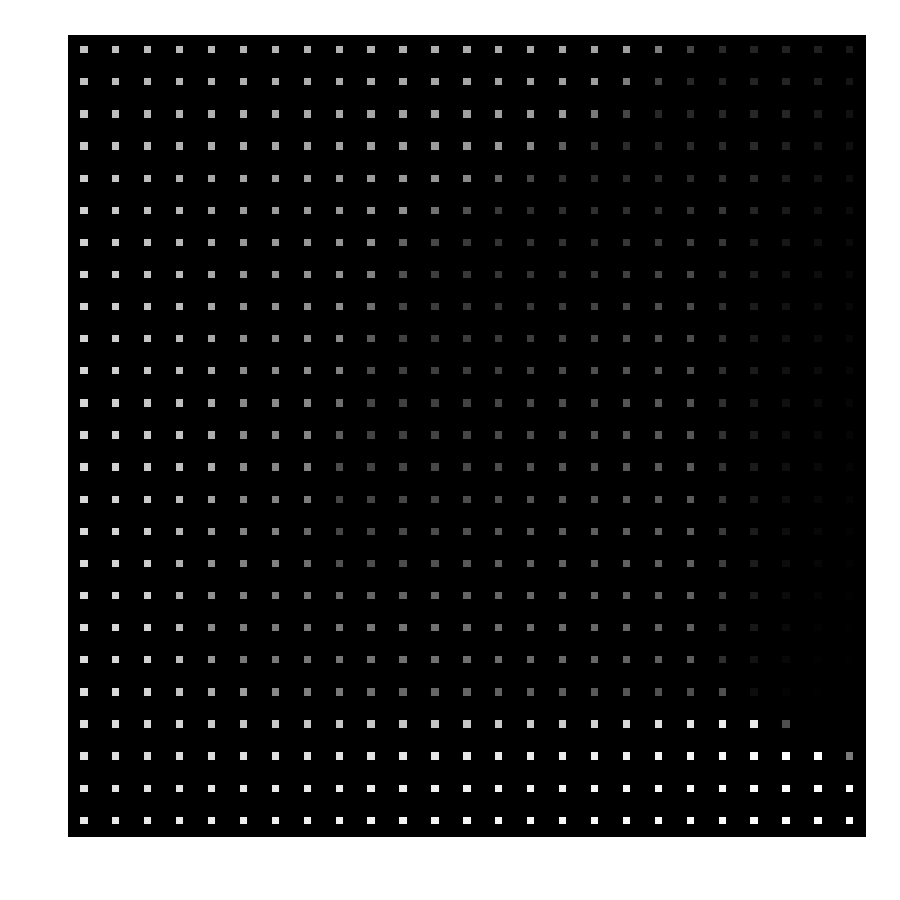
\includegraphics[width=\textwidth]{figures/deterministic_decoder}		

		
	\end{minipage}%
	\begin{minipage}{.25\textwidth}
		\centering
		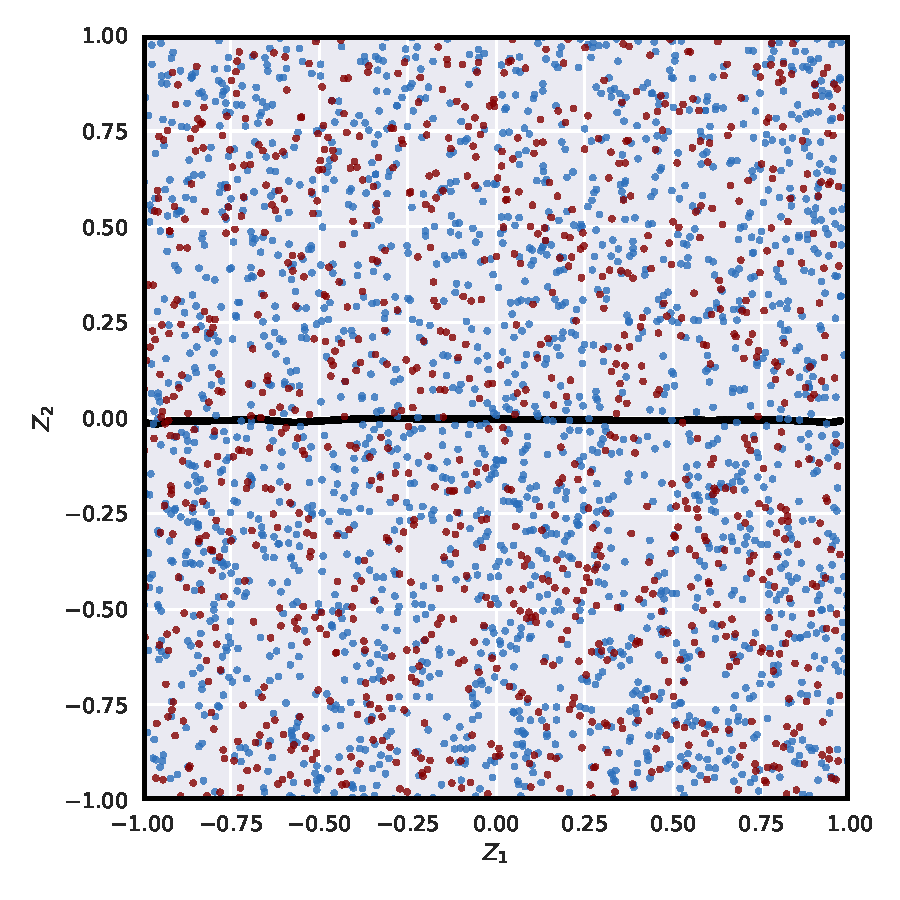
\includegraphics[width=\textwidth]{figures/random_manifold_all}	

		
	\end{minipage}%
	\begin{minipage}{.25\textwidth}
	\centering

		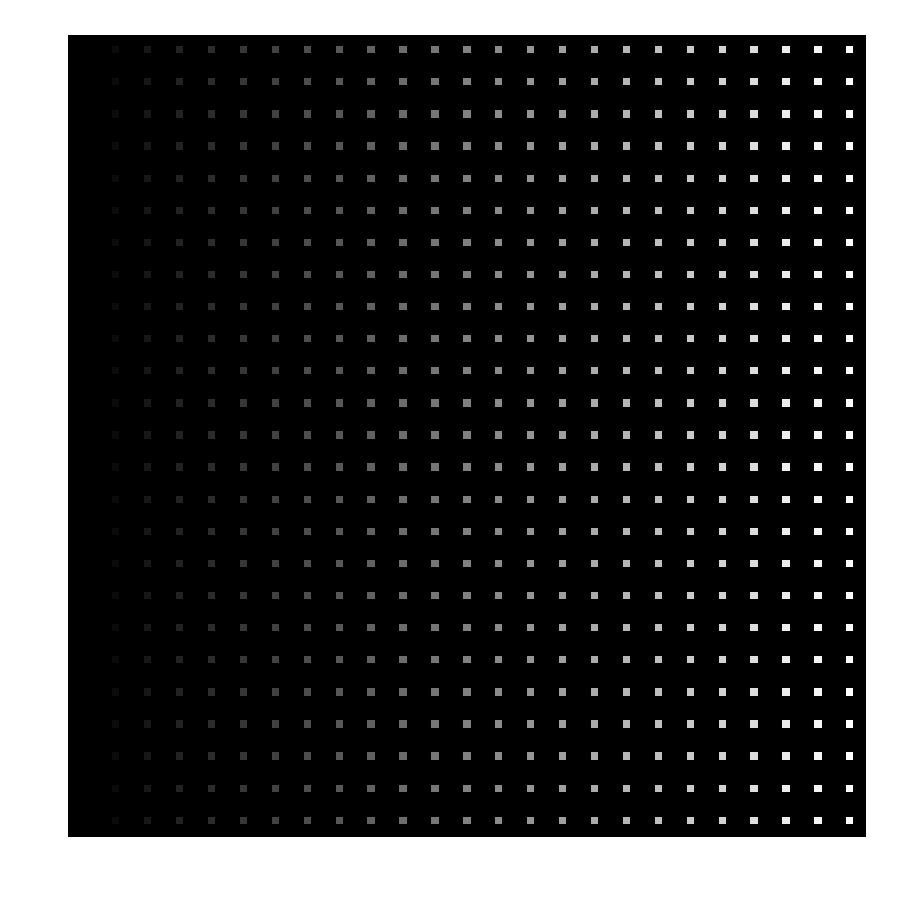
\includegraphics[width=\textwidth]{figures/random_decoder}	

\end{minipage}
	\begin{minipage}{.5\textwidth}
	\centering
	Deterministic WAE (encoder, decoder)
\end{minipage}%
	\begin{minipage}{.5\textwidth}
	\centering
	Probabilistic WAE (encoder, decoder)
\end{minipage}%
\setlength{\belowcaptionskip}{-10pt}
	\caption{\label{fig:fading-squares-latent}
		Visualisations of the 2-dimensional latent space of the WAE trained on the fading squares dataset with deterministic and probabilistic encoders and a uniform prior $P_Z$ over the box. Within each pair of plots, the left shows 1000 points sampled from the aggregated posterior $Q_Z$ ({\bf dark red}) and prior $P_Z$ ({\bf blue}); for the probabilistic encoder {\bf black} points show data points $x$ mapped to the mean values of the encoder $\E[Q(Z|X=x)]$.
		Right plots show decoder outputs at the corresponding points of the latent space.}
\end{figure*}


We repeated the same experiment with a probabilistic-encoder WAE, for which the encoder maps an input image to a uniform distribution over the axis aligned box with centre $(\varphi_{1}(x),  \varphi_{2}(x))$ and side lengths $(\sigma_{1}(x), \sigma_{2}(x))$. 
Figure \ref{fig:fading-squares-latent} (right two plots) shows the resulting behaviour of the learned encoder and decoder. In contrast to the deterministic-encoder WAE, the probabilistic-encoder WAE is robust to the fact that $\dZ > \dP$ and can use one dimension to encode useful information to the decoder while filling the other with noise. That is, a single image gets mapped to a thin and tall box in the latent space. In this way, the probabilistic-encoder WAE is able to `inflate' the latent manifold and properly match the aggregated posterior $Q_Z$ to the prior distribution $P_Z$.

To what extent is it actually a problem that the deterministic WAE represents the data as a curved manifold in the latent space? There are two issues.


\paragraph{Poor sample quality:}
Only a small fraction of the total volume of the latent space is covered by the deterministic encoder.
Hence the decoder is only trained on this small fraction, because under the objective \eqref{eq:WAEobj} the decoder learns to act only on the encoded training images. 
While it appears in this 2-dimensional toy example that the quality of decoder samples is nonetheless good everywhere, in high dimensions, such `holes' may be significantly more problematic. This possibly explains the results presented in Table \ref{table:dimension-fid-test-reconstruction}, in which we find that large latent dimensions decrease the quality of the samples produced by deterministic WAEs, and has implications for understanding the better sample quality for WAE-GAN than WAE-MMD reported in \cite{TBG+17}, discussed in Supplementary Materials \ref{appendix:wae_gan}.


\paragraph{Incorrect proportions of generated images}
Although in this toy example all of the samples generated by the deterministic-encoder WAE are of good quality, we verify empirically in Supplementary Materials \ref{appendix:wrong_proportions} that they are not produced in the correct proportions. 
By analogy, this would correspond to a model trained on MNIST producing too few 3s and too many 7s.


\subsection{\label{subsection:celebA}Probabilistic encoders with large $\dZ$}


To test our new intuitions about the behaviour of deterministic- and probabilistic-encoder WAEs with different latent dimensions, we next consider the \emph{CelebA} dataset. 
All experiments reported in this section used Gaussian priors and, for the probabilistic-encoder WAEs, Gaussian encoders. 
A~fixed convolutional architecture with cross-entropy reconstruction loss was used for all experiments. To keep computation time feasible, we used small networks.

%\vspace{-0.1cm}

Table \ref{table:dimension-fid-test-reconstruction} shows the results of training 5 probabilistic- and 5 deterministic-encoder WAEs for each value of $\dZ \in \{32, 64, 128, 256\}$. 
Deterministic- and probabilistic-encoder WAEs exhibit similar behaviour: test reconstruction error decreases as $\dZ$ increases, while the FID scores \citep{heusel2017gans} of generated samples first decrease to some minimum and then subsequently increase (lower FID scores indicate better sample quality).

%\vspace{-0.1cm}

For deterministic encoders, this agrees with the intuition we gained from the \emph{fading squares} experiment. Unable to fill the whole latent space when $\dP < \dZ$, the encoder leaves large holes in the latent space on which the decoder is never trained. When $\dP \ll \dZ$, these holes occupy most of the total volume, and thus most of the samples produced by the decoder from draws of the prior are poor.

%\vspace{-0.1cm}

For probabilistic encoders we did not expect this behaviour. We observed that the probabilistic encoders would `collapse' to deterministic encoders when $\dP\ll\dZ$, rather than using noise to expand the latent manifold, making $Q_Z$ accurately match $P_Z$. More precisely, the \emph{log-variances} for each dimension of $Q(Z|X=x)$ averaged over a mini-batch of data would typically continually decrease throughout training to less than $-20$.
%In our TensorFlow implementation we found that the collapsing variances caused numerical issues, necessitating us to clip the log-variances to lower-bound them.
%\textbf{Identifying this problem is one of the crucial points of this paper}, and we next propose a solution to this.
Identifying this problem is one of the crucial points of this paper, and we next propose a solution to this.
%The fact that this happens for most---but not all---dimensions explains why with a $256$ dimensional latent space, probabilistic-encoder WAEs produced samples with bad FID scores, but still better than deterministic-encoder WAEs: to some extent dimesionality reduction \emph{does} occur, just not as much as we would hope for.

	\begin{table}[t!]
	\caption{FID scores and test reconstructions for deterministic- and probabilistic-encoder WAEs trained on \emph{CelebA} for various latent dimensions $\dZ$. Test reconstructions get better with increased dimension, while FID scores suffer for $\dZ \gg \dI$.}
	\label{table:dimension-fid-test-reconstruction}
	\vskip 0.15in
	\begin{center}
		\begin{small}
			\begin{sc}
				\resizebox{0.7\columnwidth}{!}{%
					\begin{tabular}{lcccccr}
						\toprule
						$\dZ$ & \multicolumn{2}{c}{FID score} & \multicolumn{2}{c}{Test reconstruction} \\
						&  Det. & Prob.  & Det. & Prob.\\
						\midrule
						32    & 75.0$\pm$ 0.7& 74.8$\pm$ 0.5& 6457.0$\pm$ 10.4& 6445.5$\pm$ 7.5 \\
						64 & 71.6 $\pm$ 0.8 & 71.1 $\pm$ 1.0 & 6364.4$\pm$ 7.4 & 6365.0$\pm$ 5.4 \\
						128    & 76.8$\pm$ 1.3& 76.8$\pm$ 1.2& 6300.5$\pm$ 6.6& 6309.3$\pm$ 9.7 \\
						256    & 147.6$\pm$ 2.3& 139.8$\pm$ 4.2&6265.3$\pm$ 9.5& 6262.6$\pm$ 6.7    \\
						\bottomrule
				\end{tabular}}
			\end{sc}
		\end{small}
	\end{center}
	\vskip -0.1in
\end{table}	

\vspace{0.5cm}

\paragraph{Resolving variance collapse through regularization}\label{section:L1_reg}
The precise cause of this variance collapse is uncertain to us. 
It is clear that the reconstruction loss will encourage small variances (since this makes the task of the decoder easier), and we suspect that the MMD fails to prevent this from happening due to the weakness of the topology on distributions it induces as a distance.

Nonetheless, we found we could effectively eliminate this issue by adding an $L_p$ penalty on the log-variances,   providing encouragement for the variances to remain closer to $1$ and thus for the encoder to remain stochastic. More precisely, we added the following term to the objective function to be minimised:
%\begin{align}
%\resizebox{0.9\textwidth}{!}{
%$\displaystyle
%\frac{1}{N} \sum_{n=1}^N c(x_n, G_\theta(z_n)) + 
% \lambda \left(\frac{\sum_{n\not=m} k(z_n, z_m) }{N(N-1)} + \frac{\sum_{n\not=m} k(\tilde{z}_n, \tilde{z}_m)}{N(N-1)} - \frac{2\sum_{n,m} k(z_n, \tilde{z}_m) }{N^2}\right)   + {\color{blue}\frac{\lambda_{p}}{N}\sum_{n=1}^N \sum_{i=1}^{\dZ} \left|\log\left(\sigma^2_{i}(x_n)\right) \right|^p}
%$
% }
%\end{align}
\begin{equation}
\frac{\lambda_{p}}{N}\sum_{n=1}^N \sum_{i=1}^{\dZ} \left|\log\left(\sigma^2_{i}(x_n)\right) \right|^p
\end{equation}

%\begin{align}
%\begin{split}
%\frac{1}{N} \sum_{n=1}^N c(x_n, G_\theta(z_n)) + 
%& \lambda \left(\frac{\sum_{i\not=j} k(z_i, z_j) }{N(N-1)} + \frac{\sum_{i\not=j} k(\tilde{z}_i, \tilde{z}_j)}{N(N-1)} - \frac{2\sum_{i,j} k(z_i, \tilde{z}_j) }{N^2}\right)
%\\
%& \qquad \qquad \qquad \qquad \qquad + \frac{\lambda_{p}}{N}\sum_{n=1}^N \sum_{i=1}^{\dZ} \left|\log\left(\sigma^2_{i}(x_n)\right) \right|^p
%\end{split}
%\end{align}

% \widehat{MMD}_k\left(\{z_n\}, \{\tilde{z}_n\}\right)

where  $i$ indexes the dimensions of the latent space $\Z$, $n$ indexes the inputs $x_n$ in a mini-batch, and $\lambda_{p}\geq 0$ is the new regularization coefficient.

We experimented with both $L_1$ and $L_2$ regularisation and found both to give similar qualitative behaviour, but $L_1$ regularisation gave better performance and thus we report only these results. There are two interpretations we have for why $L_1$ regularisation might be sensible.

First, note that an $L_1$ penalty on the log-variances should encourage the encoder/decoder pair to \emph{sparsely} use latent dimensions to code useful information. Indeed, the $L_1$ penalty will encourage sparsely many dimensions to have non-zero log-variances, and if the variance of $Q(Z_i|X)$ in some dimension $i$ is always $1$ then in order for the marginal $Q_Z(Z_i)$ to match $P_Z(Z_i)$, we must have that $\varphi_i(x)=0$ for all inputs $x$, meaning that $\varphi_i(X)$ contains no information about $X$.

\begin{figure*}[t!]
	\centering
	\begin{minipage}{.02\textwidth}
		\begin{turn}{90}
			\hspace{1cm} $\dZ =256$\hspace{3.5cm} $\dZ =32$\hspace{1cm}
		\end{turn}       
	\end{minipage}
	\begin{minipage}{.45\textwidth}
		\centering
		(a) Test reconstruction vs $L_1$ regularisation
		\begin{tikzpicture}
		\node[anchor=south west,inner sep=0] (image) at (0,0) {		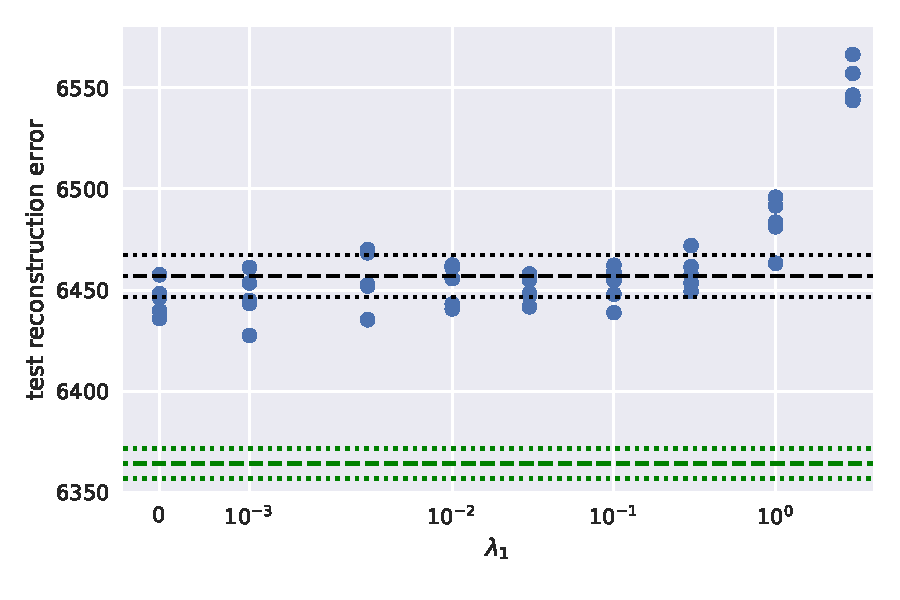
\includegraphics[width=\columnwidth]{figures/celebA_errors_vs_L1_32}};
		\begin{scope}[x={(image.south east)},y={(image.north west)}]
		\draw[thick, red] (0.177,0.81) -- (0.177,0.56){};
		\node (recon32) at (0.27,0.845) {
			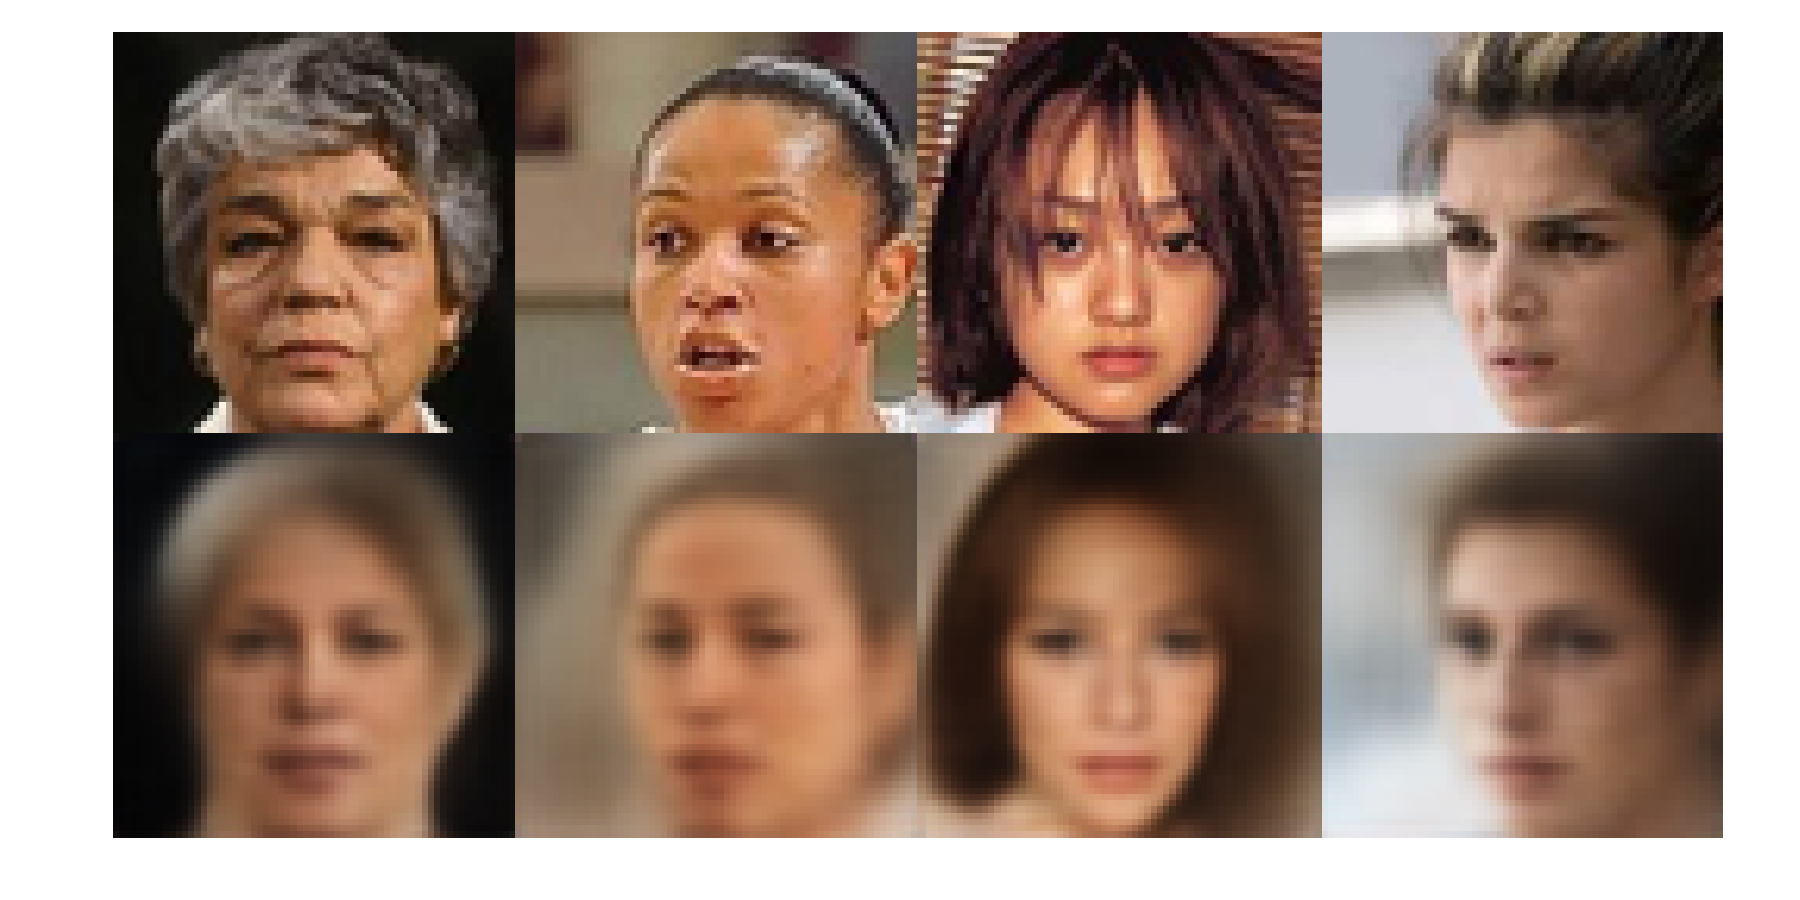
\includegraphics[width=0.3\columnwidth]{figures/recons_32_0_many_h}};
		\draw[red, thick,rounded corners] (0.177,0.543) circle (0.1cm);
		\draw[thick, red] (0.72,0.877) -- (0.9362,0.877){};
		\node (recon32) at (0.7,0.845) {
			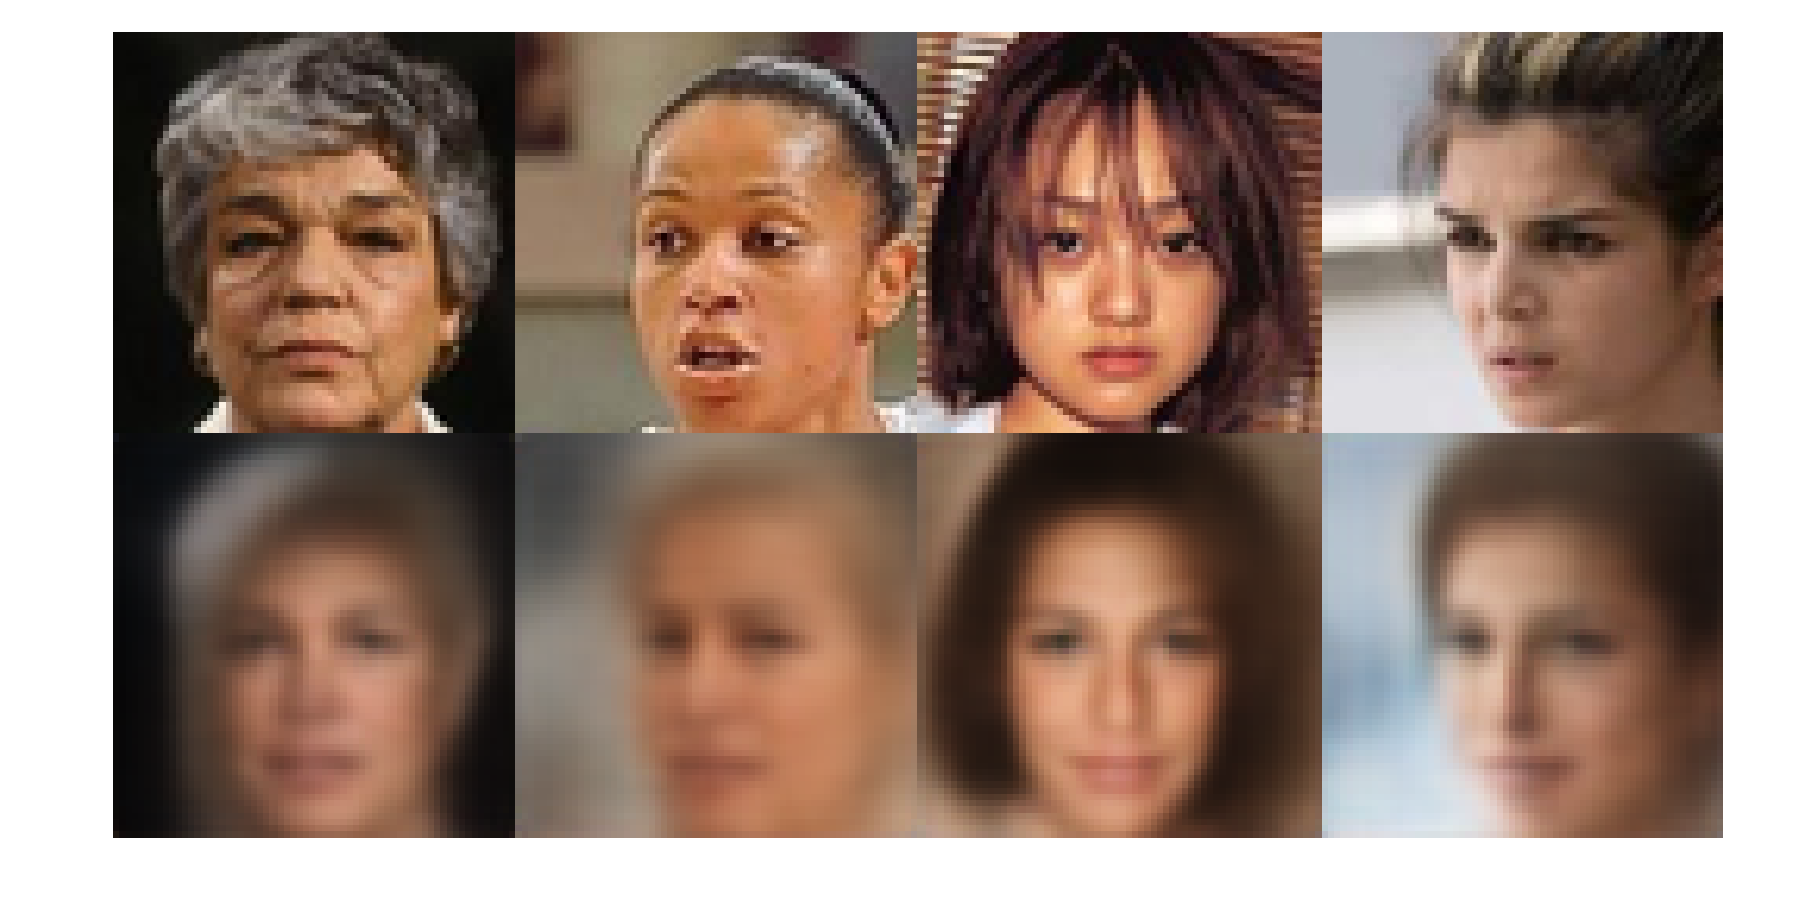
\includegraphics[width=0.3\columnwidth]{figures/recons_32_3_many_h}};
		\draw[red, thick,rounded corners] (0.947,0.877) circle (0.1cm);
		\end{scope}
		\end{tikzpicture}
		
		\begin{tikzpicture}
		\node[anchor=south west,inner sep=0] (image) at (0,0) {		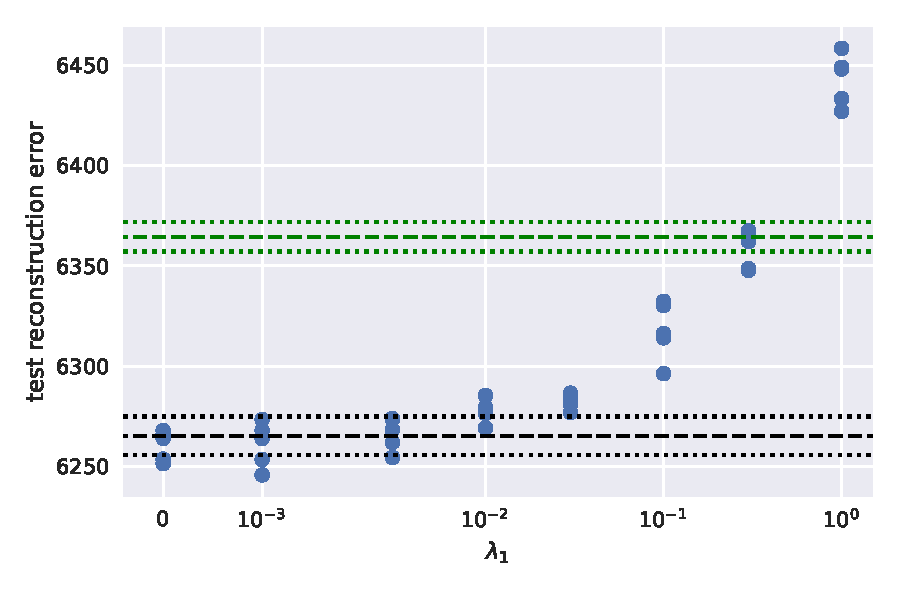
\includegraphics[width=\columnwidth]{figures/celebA_test_error_vs_L1_256}};
		\begin{scope}[x={(image.south east)},y={(image.north west)}]
		\draw[thick, red] (0.182,0.81) -- (0.182,0.31){};
		\node (recon32) at (0.27,0.845) {
			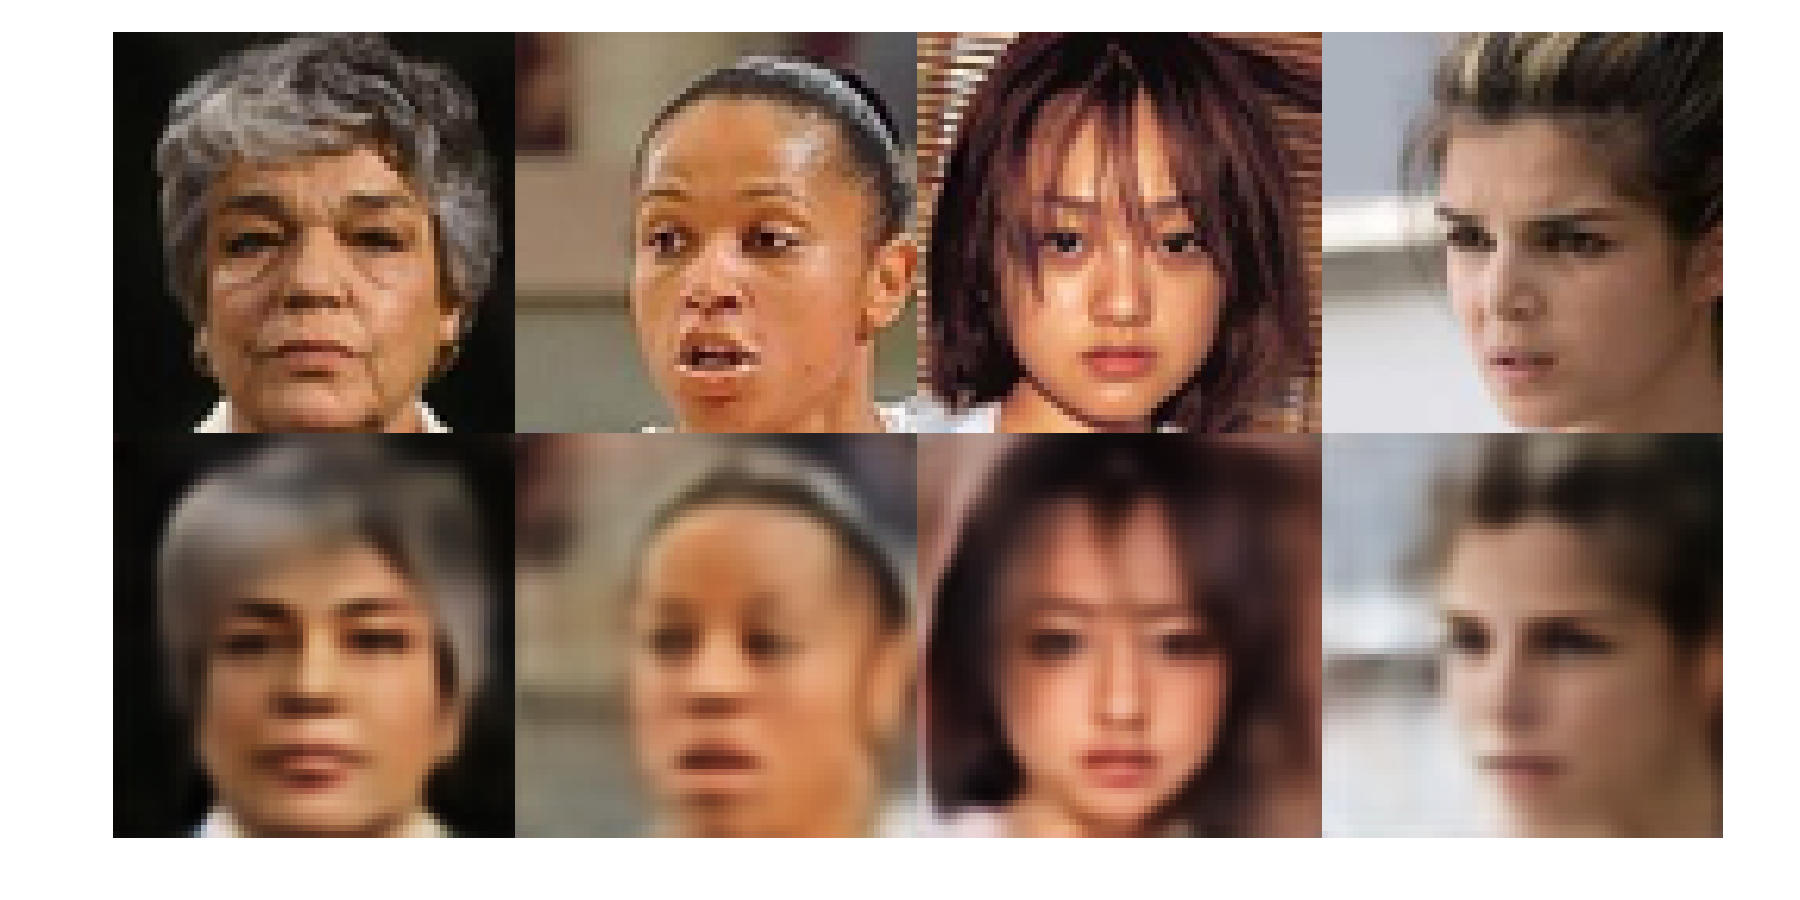
\includegraphics[width=0.3\columnwidth]{figures/recons_256_0_many_h}};
		\draw[red, thick,rounded corners] (0.182,0.28) circle (0.15cm);
		\draw[thick, red] (0.737,0.885) -- (0.737,0.52){};
		\node (recon32) at (0.7,0.845) {
			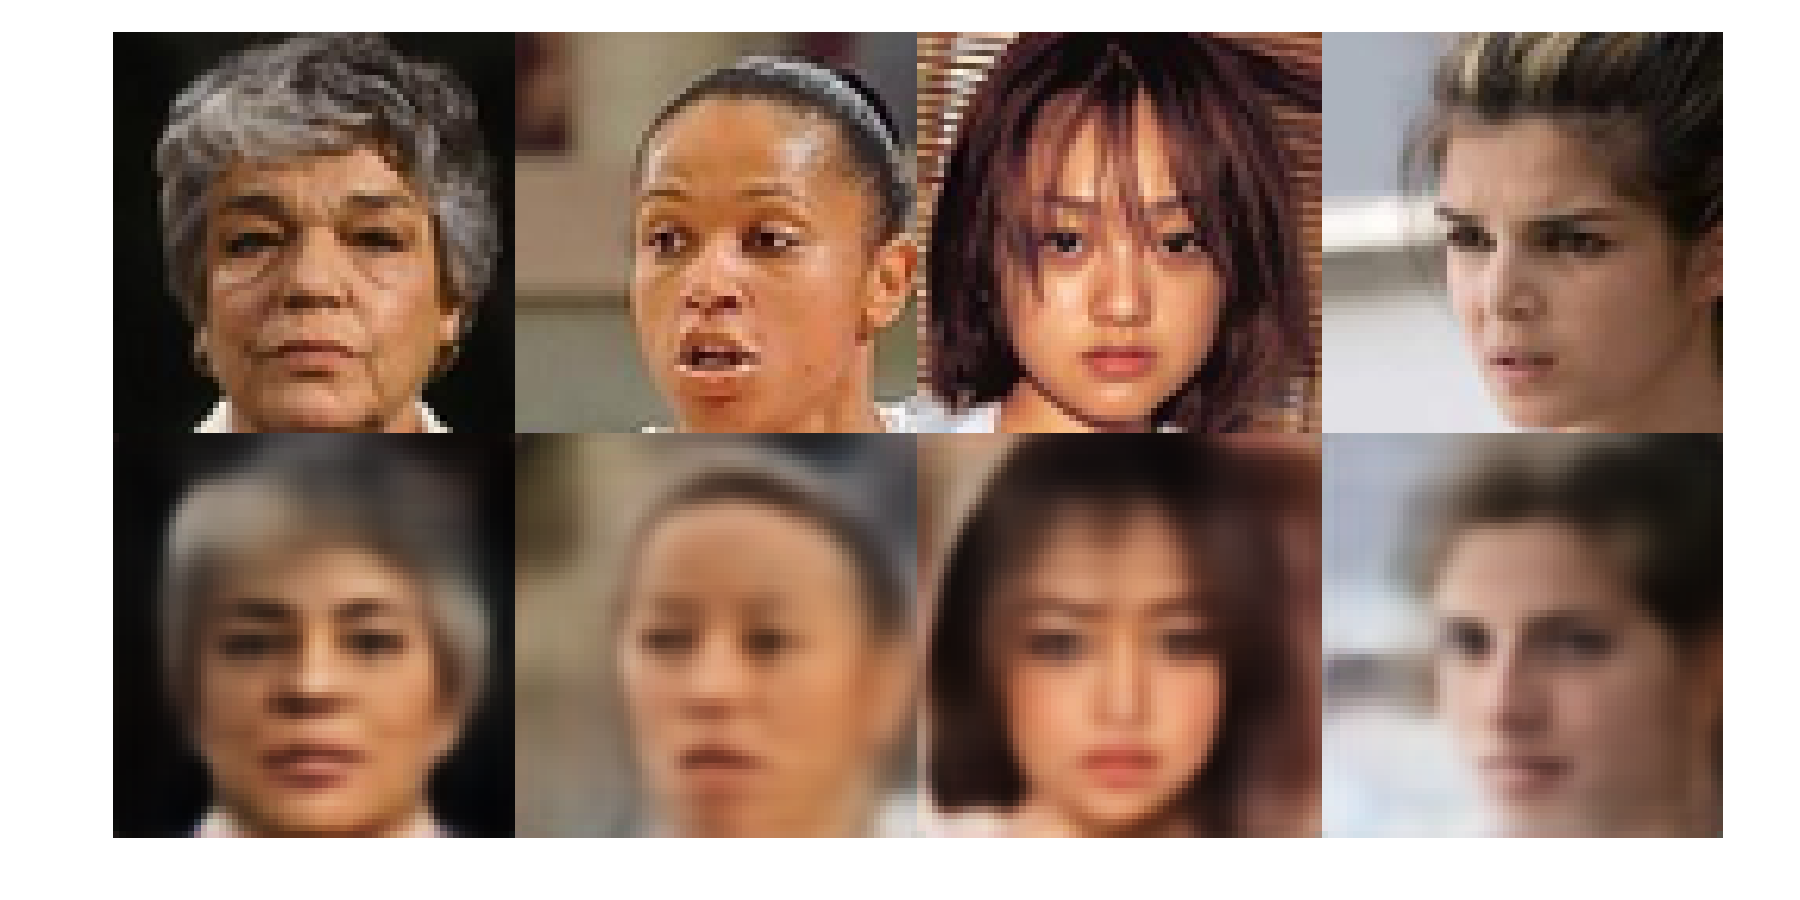
\includegraphics[width=0.3\columnwidth]{figures/recons_256_01_many_h}};
		\draw[red, thick,rounded corners] (0.737,0.498) circle (0.13cm);
		\end{scope}
		\end{tikzpicture}
		
		
		
	\end{minipage}%
	\begin{minipage}{.45\textwidth}
		\centering
		(b) FID scores vs $L_1$ regularisation
		
		\begin{tikzpicture}
		\node[anchor=south west,inner sep=0] (image) at (0,0) {		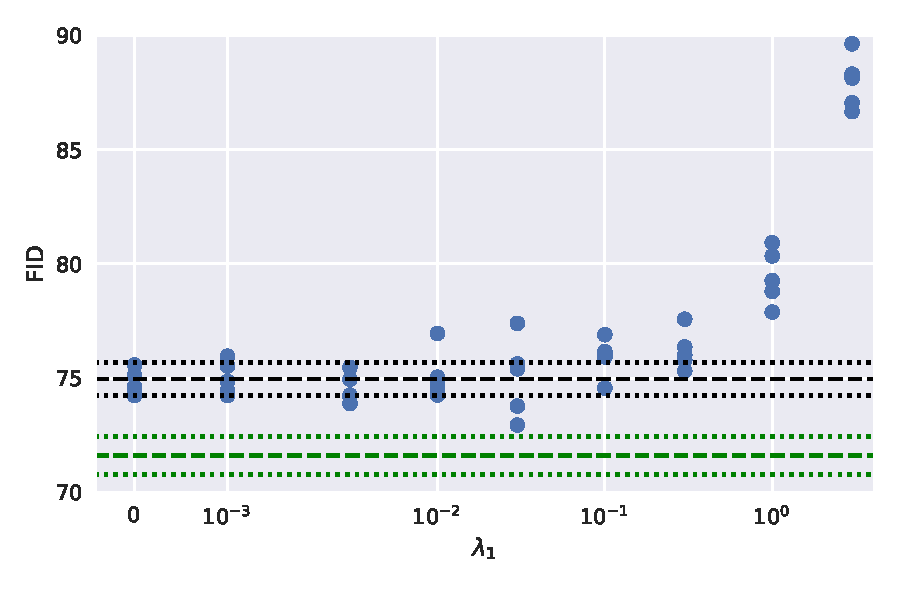
\includegraphics[width=\columnwidth]{figures/celebA_FID_vs_L1_32}};
		\begin{scope}[x={(image.south east)},y={(image.north west)}]
		\draw[thick, red] (0.15,0.81) -- (0.15,0.415){};
		\node (recon32) at (0.25,0.83) {
			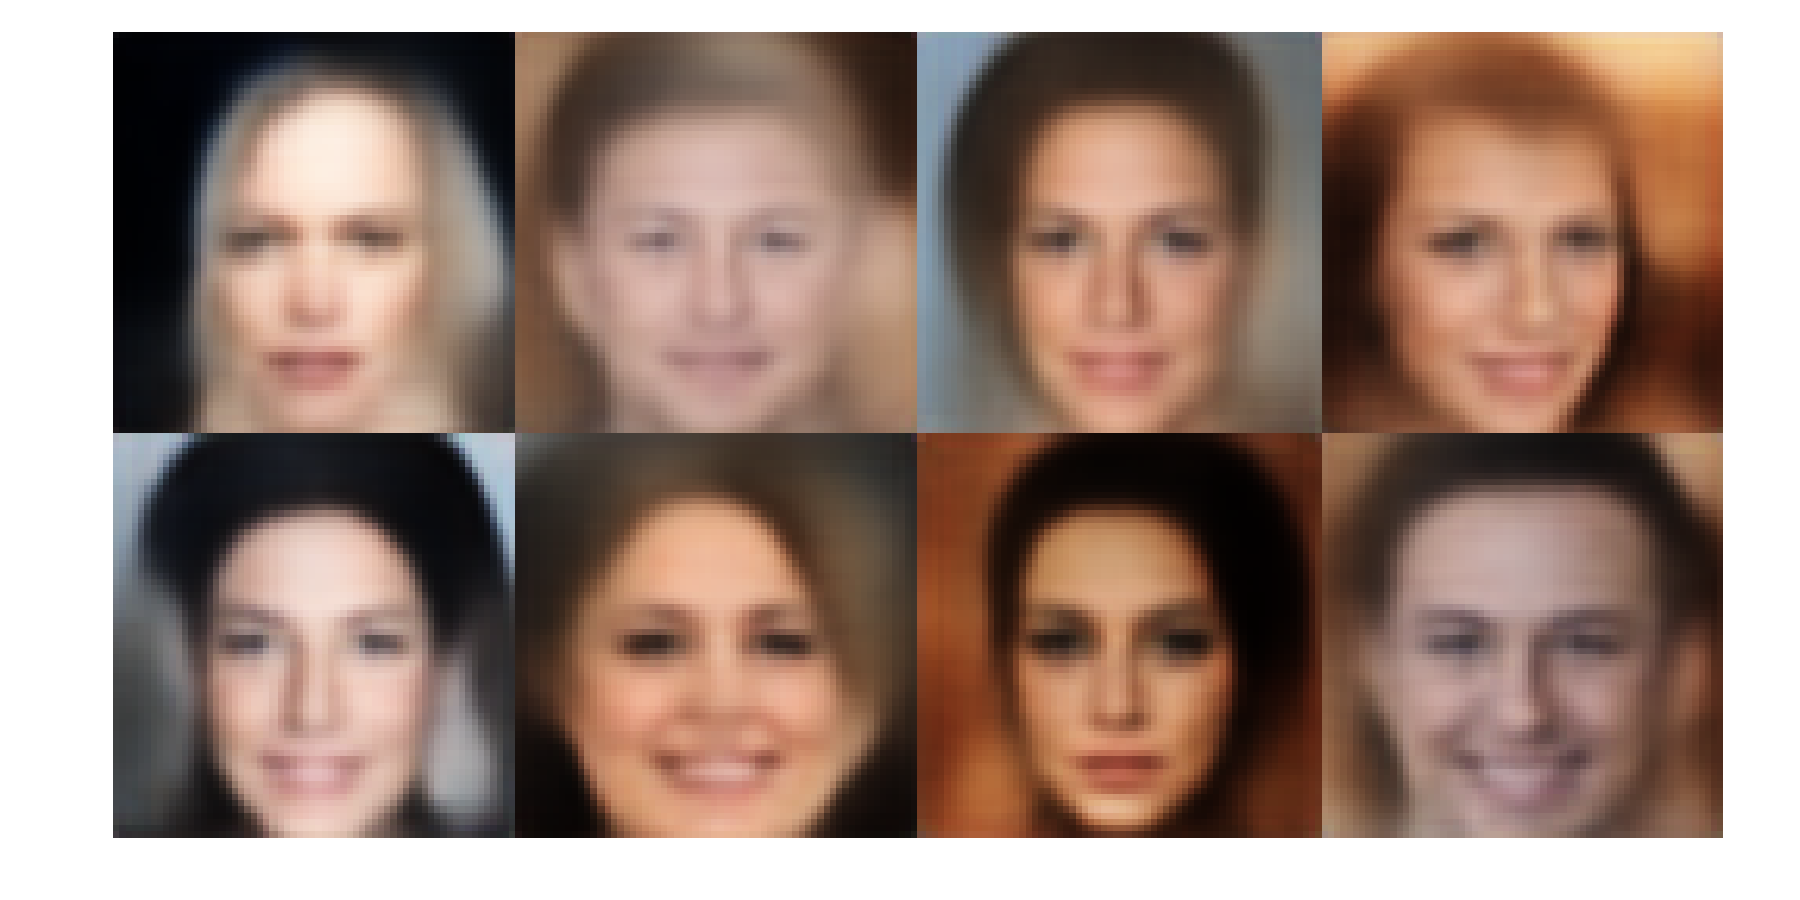
\includegraphics[width=0.3\columnwidth]{figures/samples_32_0_many_h}};
		\draw[red, thick,rounded corners] (0.15,0.39) circle (0.13cm);
		\draw[thick, red] (0.72,0.876) -- (0.928,0.876){};
		\node (recon32) at (0.7,0.83) {
			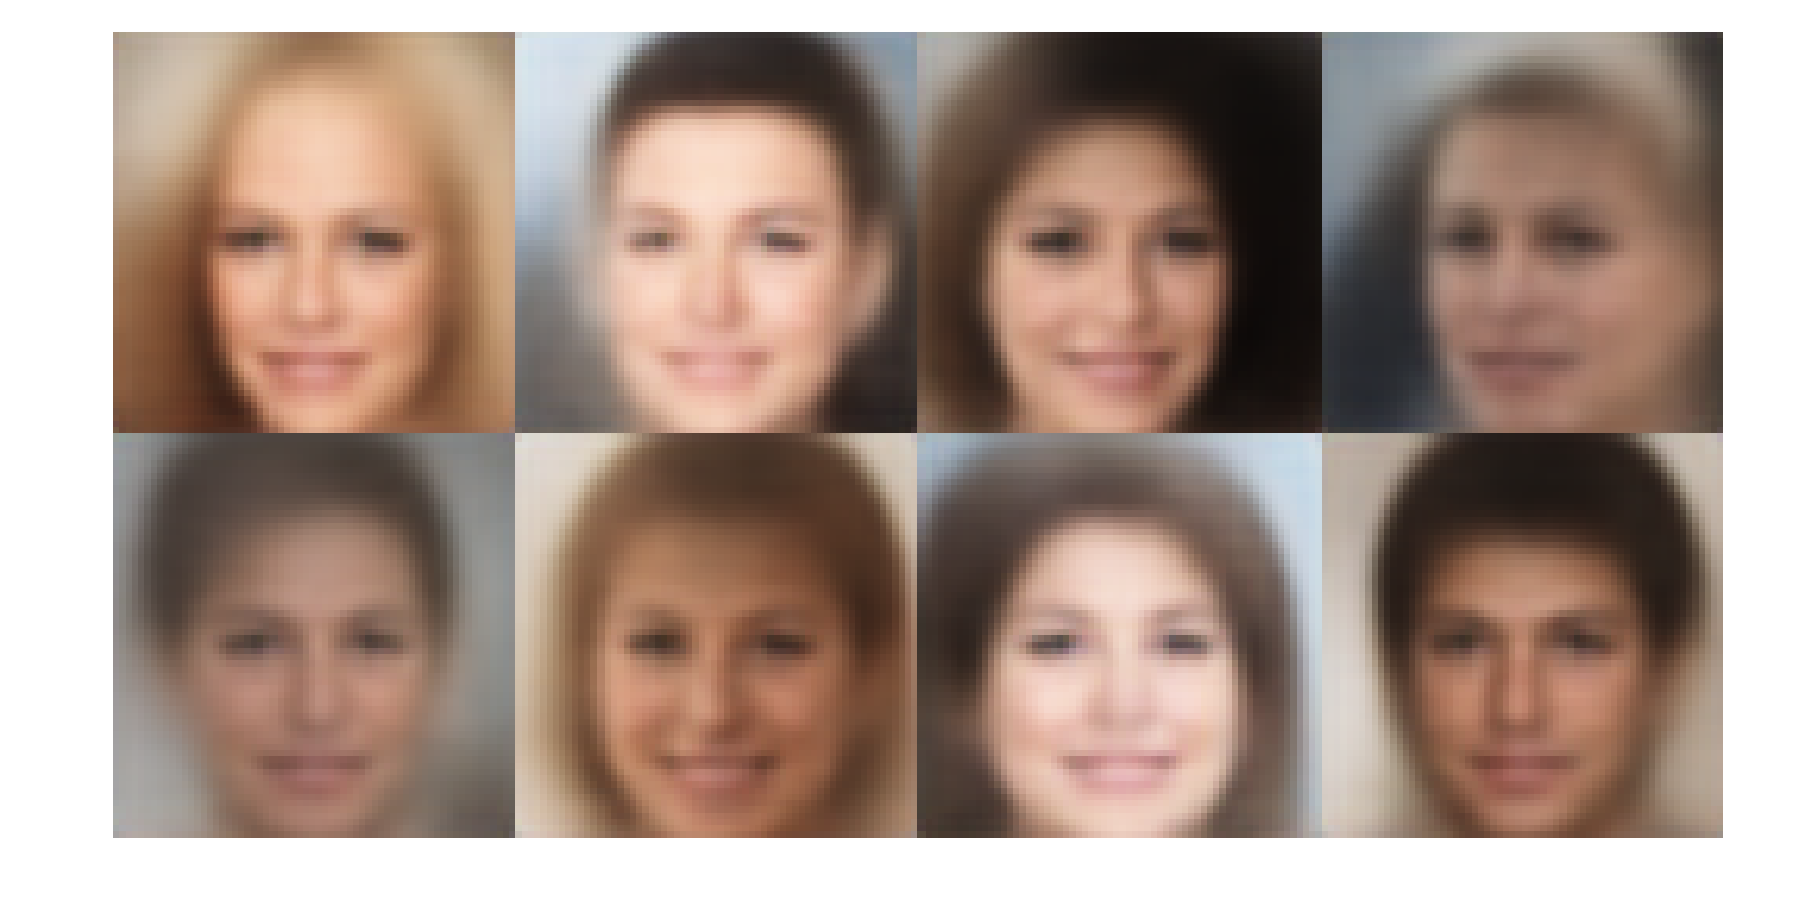
\includegraphics[width=0.3\columnwidth]{figures/samples_32_3_many_h}};
		\draw[red, thick,rounded corners] (0.946,0.876) circle (0.15cm);
		\end{scope}
		\end{tikzpicture}
		
		\begin{tikzpicture}
		\node[anchor=south west,inner sep=0] (image) at (0,0) {		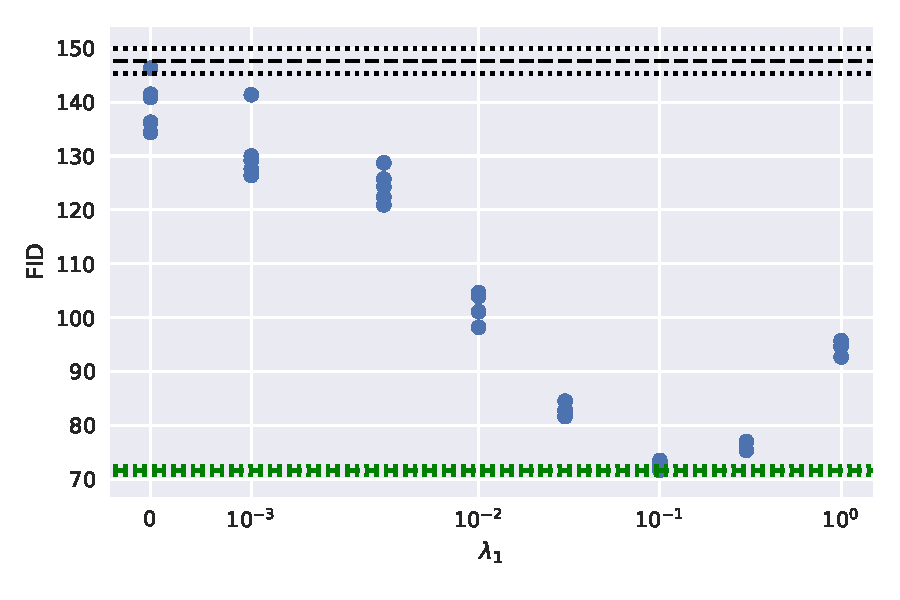
\includegraphics[width=\columnwidth]{figures/celebA_FID_vs_L1_256}};
		\begin{scope}[x={(image.south east)},y={(image.north west)}]
		\draw[thick, red] (0.168,0.758) -- (0.168,0.415){};
		\node (recon32) at (0.265,0.4) {
			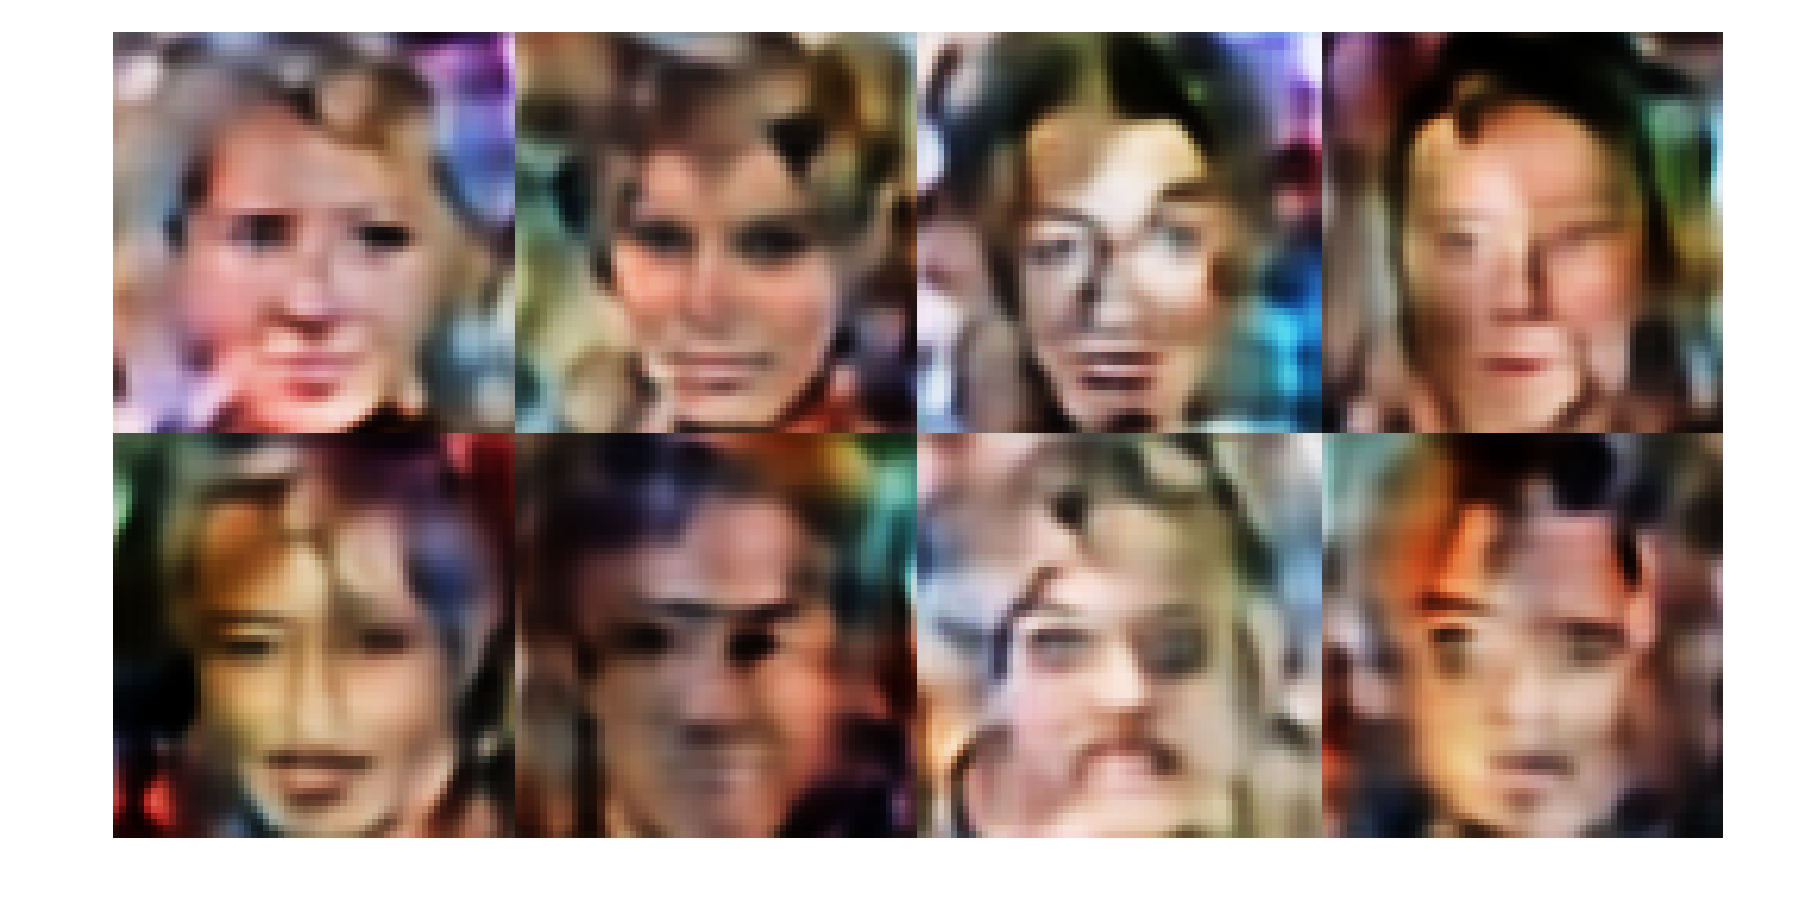
\includegraphics[width=0.3\columnwidth]{figures/samples_256_0_many_h}};
		\draw[red, thick,rounded corners] (0.168,0.78) circle (0.1cm);
		\draw[thick, red] (0.732,0.73) -- (0.732,0.255){};
		\node (recon32) at (0.73,0.73) {
			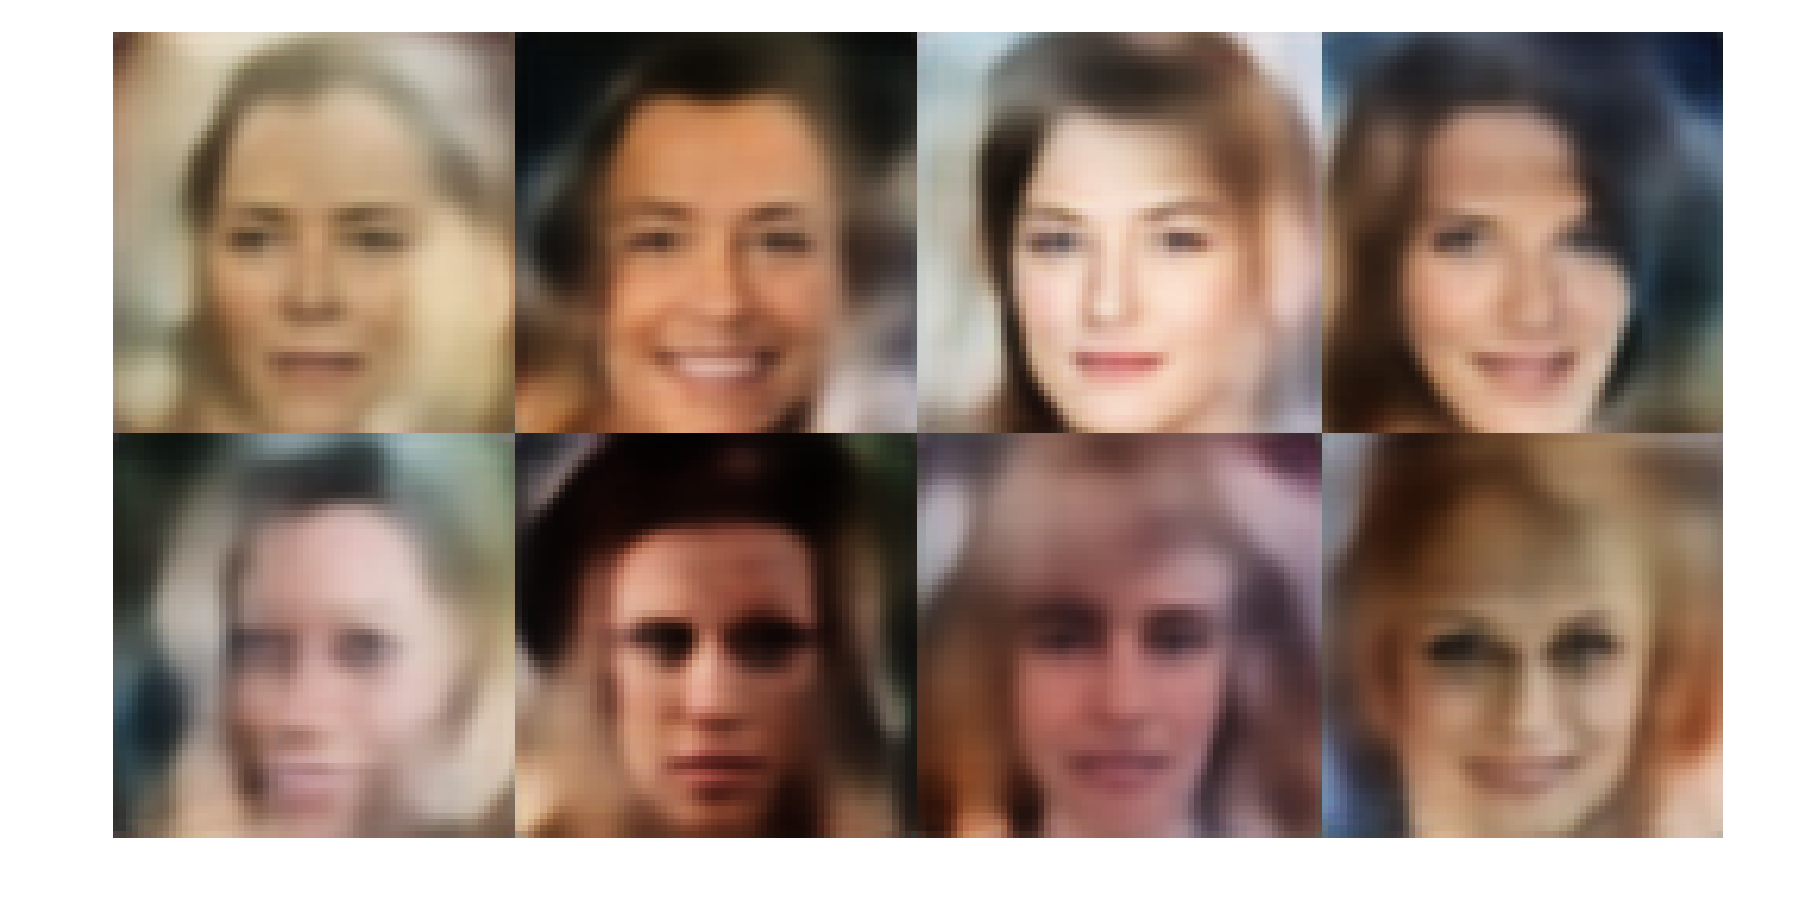
\includegraphics[width=0.3\columnwidth]{figures/samples_256_01_many_h}};
		\draw[red, thick,rounded corners] (0.732,0.225) circle (0.15cm);
		\end{scope}
		\end{tikzpicture}
		
		
		
		
	\end{minipage}%
	\caption{\label{fid:celebA-fid-test-errors-vs-latent-dim}FID scores and test reconstruction errors for probabilistic-encoder WAEs with latent space dimension $\dZ=32$ (\textbf{first row}) and $\dZ=256$ (\textbf{second row}) for different $L_1$ regularisation coefficients $\lambda_1$. In each plot, the dashed/dotted black lines represent the mean $\pm$ s.d. for deterministic-encoder WAEs with the same $\dZ$ (i.e. $32$ or $256$). The dashed/dotted green lines represent the mean $\pm$ s.d. for deterministic WAEs $\dZ=64$, for which the FID scores were best amongst all latent dimensions we tested. Overlaid images are (a) test reconstructions and (b) random samples coming from experiments indicated by the red circle. These plots show that when $\dZ<\dP$, (i) probabilistic-encoder WAEs perform comparably to deterministic WAEs and (ii) when appropriately regularised ($\lambda=10^{-1}$), probabilistic encoders with high dimensional latent spaces can produce samples of similar quality to deterministic encoders with tuned latent dimension. At the same time, the test reconstruction errors are lower.}
\end{figure*}


The second interpretation of this term comes from the observation that $|\log\left(\sigma^2 \right)|$ and $\sigma^2  - \log\left(\sigma^2\right)$ both attain their minimum at $\sigma^2=1$. The first term is our regulariser, while the second term is the log-variance part of the KL regulariser of the VAE objective. In this sense, our new objective is related to that of DIP-VAE \citep{kumar2017variational}, which takes the VAE objective and adds a term to penalise a divergence $D(P_Z, Q_Z)$.

Using latent dimensions 32 and 256 to consider both the case of under- and over-shooting the intrinsic dimensionality of the dataset,\footnote{The fact that the deterministic WAE produced samples with better FIDs with $\dZ=64$ than $\dZ=32$ suggested to us that the intrinsic dimensionality of the CelebA datset is greater than 32.} we trained 5 $L_1$-regularized probabilistic-encoder WAEs for a variety of values for $\lambda_1$. Figure \ref{fid:celebA-fid-test-errors-vs-latent-dim} shows the test reconstruction errors and FID scores obtained at the end of training.

When $\dZ$ is large, $L_1$ regularisation can significantly improve the performance of probabilistic-encoder WAEs as measured by FID scores compared to their deterministic counterparts. In particular, tuning for the best $\lambda_1$ parameter results in samples of quality comparable to deterministic encoders with the best latent dimension size, while simultaneously achieving lower test reconstruction errors.
Through appropriate regularisation, probabilistic-encoder WAEs are able to adapt to large $\dZ$ and still perform well.

When $\dZ < \dI$,  $L_1$ regularisation does not improve test reconstruction error and FID scores and the probabilistic-encoder WAEs perform at best the same as deterministic-encoder WAEs. This makes sense: if in the deterministic case the WAE is already having to perform `lossy compression' by reducing the effective dimensionality of the dataset, then the optimal probabilistic encoder cannot do better than becoming deterministic. Thus, forcing the encoder to be more random can only harm performance.

%Taking a step back, it would be a valid comment to suggest that we have merely substituted the problem of searching for the `right' latent dimensionality $\dZ$ with the problem of searching for the `right' regularisation $\lambda_1$. 
%Our longer-term view is that 

We have demonstrated a way to train probabilistic-encoder WAEs without collapsing to deterministic encoders.
In doing so we have provided a way of making WAEs capable of adapting to the intrinsic data dimensionality.
 However, it could be argued that our approach merely substitutes the problem of searching for the `right' latent dimensionality $\dZ$ with the problem of searching for the `right' regularisation $\lambda_1$. 
Future directions of research include exploring divergence measures other than MMD and whether the $L_p$ regularisation coefficients $\lambda_p$ can be adaptively adjusted by the learning machine itself.

\vspace{-0.2cm}

\section{\label{section:disentanglement}Learned representation and disentanglement}

\vspace{-0.2cm}

%\begin{figure*}[t]
%	\centering
%	\begin{subfigure}[t]{0.5\textwidth}
%		\centering
%		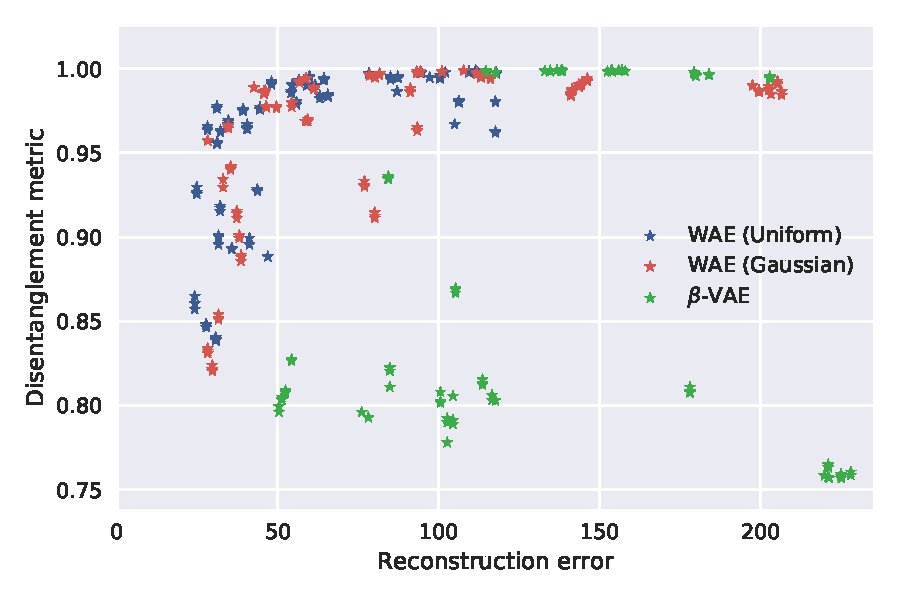
\includegraphics[width=\columnwidth]{figures/main_paper_reconstruction_error_vs_disentanglement_4}
%		\caption{\label{subfig:disentanglement-vs-reconstruction-4}4-variable \emph{dSprites} disentanglement task.}
%	\end{subfigure}%
%	~ 
%	\begin{subfigure}[t]{0.5\textwidth}
%		\centering
%		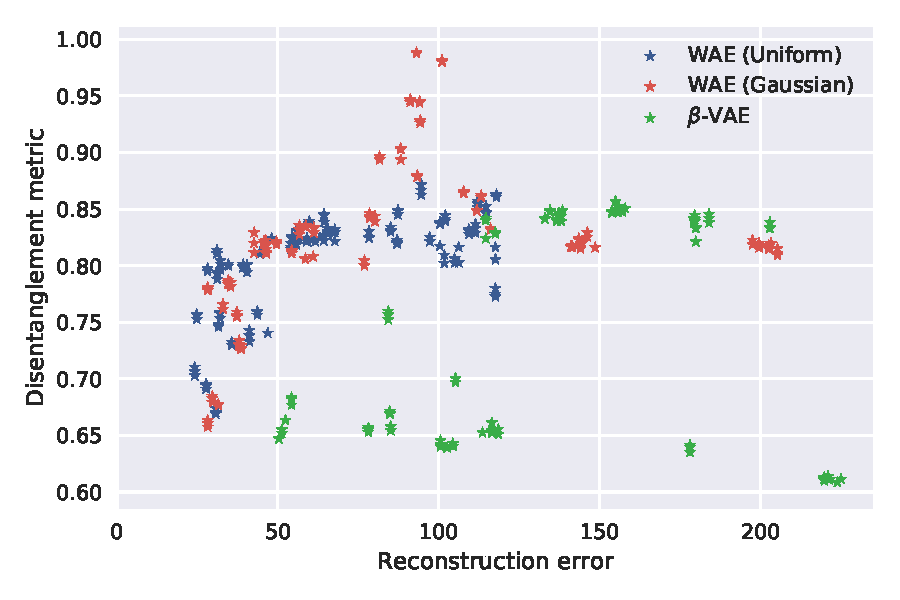
\includegraphics[width=\columnwidth]{figures/main_paper_reconstruction_error_vs_disentanglement_5}
%		\caption{\label{subfig:disentanglement-vs-reconstruction-5}5 variable \emph{dSprites} disentanglement task.}
%	\end{subfigure}
%	\caption{\label{fig:disentanglement-vs-reconstruction}Disentanglement vs reconstruction error for $\beta$-VAEs with various values of $\beta$ and WAEs with various $L_1$ regularisation coefficients $\lambda_1$ \textbf{(up and left is better)}. Note that there is no direct way to compare different values of $\beta$ and $\lambda_1$, but in both cases increasing the value of the hyper-parameter is correlated with increasing reconstruction error. \textbf{WAEs are capable of achieving comparable or better disentanglement scores than the $\beta$-VAE while simultaneously achieving lower reconstruction errors.} In particular, WAE attains a maximum $\mathbf{98.8\%}$ on the 5-variable disentanglement tast, compared to a maximum of $\mathbf{85.4\%}$ for $\beta$-VAE)}
%\end{figure*}

\emph{Disentangled representation learning} is closely related to the more general problem of \emph{manifold learning} for which auto-encoding architectures are often employed. The goal, though not precisely defined, is to learn representations of datasets such that individual coordinates in the feature space correspond to human-interpretable generative factors  (also referred to as \emph{factors of variation} in the literature). It is argued by \citet{bengio2013representation} and \citet{lake2017building} that learning such representations is essential for significant progress in machine learning research.

Recently, \citet{HM+17} proposed the synthetic \emph{dSprites} dataset and a metric to evaluate algorithms on their ability to learn disentangled representations. The dataset consists of $2$-dimensional white shapes on a black background with $5$ factors of variation: shape, size, rotation, $x$-position and $y$-position. 

The proposed metric assumes ground truth labels for the generative factors are given. We provide here an intuition of what the metric does; see \citet{HM+17} for full details. Given a trained feature map $\varphi\colon \X\to\Z$ from the image space to the latent space, we ask the following question. Suppose we are given two images $x_1$ and $x_2$ which have exactly one latent factor whose value is the same---say they are both the same shape, but different in size, position and rotation. 
By looking at the \emph{absolute values of the difference in feature vectors} ${|\varphi(x_1) - \varphi(x_2)|}\in\R^{\dZ}$, is it possible to identify that it is the \emph{shape} that they share in common, and not any other factor? 

\cite{kim2018disentangling} point out that the metric of \cite{HM+17} has a failure mode: it is possible to attain 100\% accuracy with this metric without having representations of all the generative factors. They propose a modified version of this metric that does not exhibit this failure mode. 

\cite{kumar2017variational} propose yet another disentanglement metric, based on the linear correlation between generative factors and feature coordinates. Under their metric, a feature map scores highly if each generative factor is highly correlated with one feature coordinate, and uncorrelated with the rest.

Each of these three papers additionally proposes a model based on a modification to the VAE objective. The $\beta$-VAE of \cite{HM+17} multiplies the KL regulariser by a scalar $\beta$. 
FactorVAE of \cite{kim2018disentangling} augments the ELBO by adding a \emph{Total Correlation} penalty encouraging $Q_Z$ to be factorised, which is estimated adversarially. 
DIP-VAE of \cite{kumar2017variational} adds a term similar to the WAE regulariser, penalising a divergence $D(Q_Z, P_Z)$. 
Two different choices of divergence give rise to DIP-VAE-i and DIP-VAE-ii.
In all of these cases the objective function is still a lower bound on the marginal log-likelihood, provided that the additional term is non-negative.

Given these metrics, we have a well-defined task: learn representations that score highly on each metric while simultaneously achieving low test reconstruction. 
The additional regularisers for each model encourage disentanglement in the learned representation, but in practice increase test reconstruction error since they further constrain the auto-encoder.
%
\begin{figure}[t]
	\centering
	\begin{subfigure}[t]{0.33\textwidth}
		\centering
		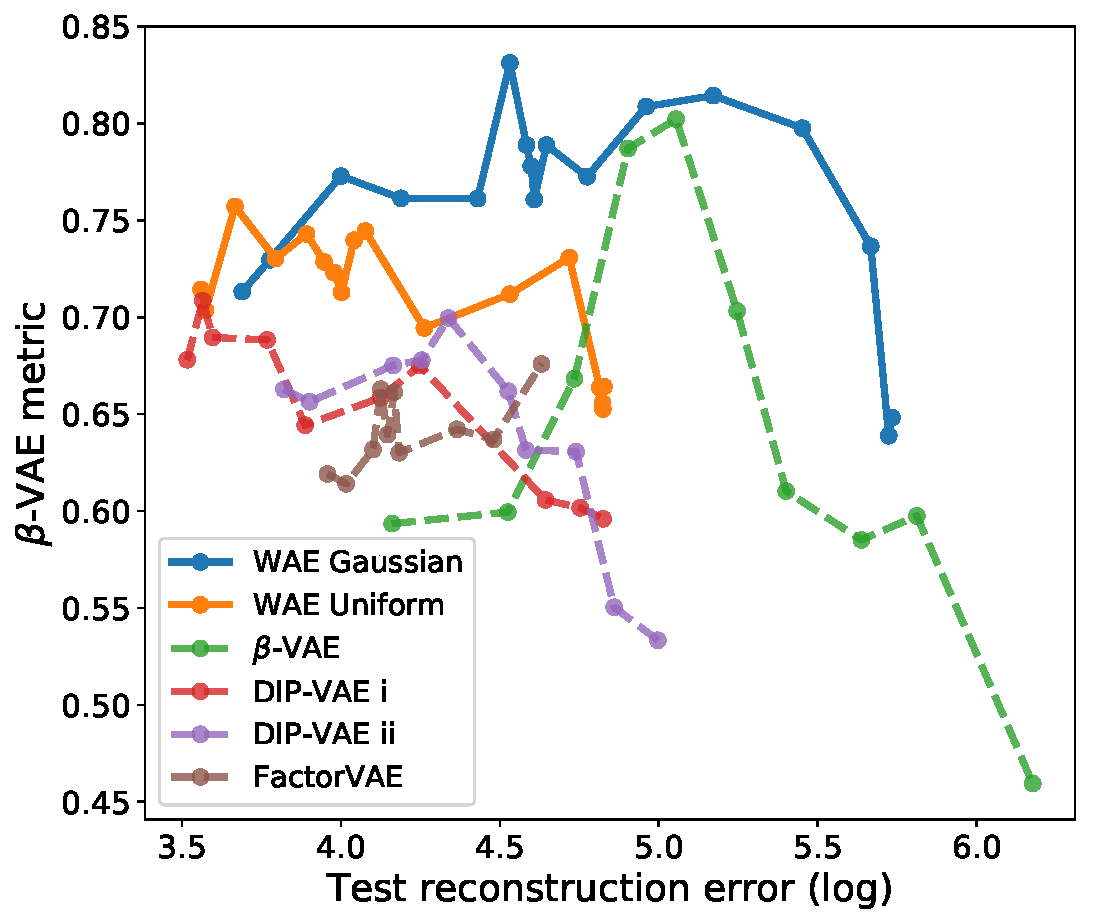
\includegraphics[width=\columnwidth]{figures/subset_beta_VAE_5_avg_b}
		\caption{}
	\end{subfigure}%
	~ 
	\begin{subfigure}[t]{0.33\textwidth}
		\centering
		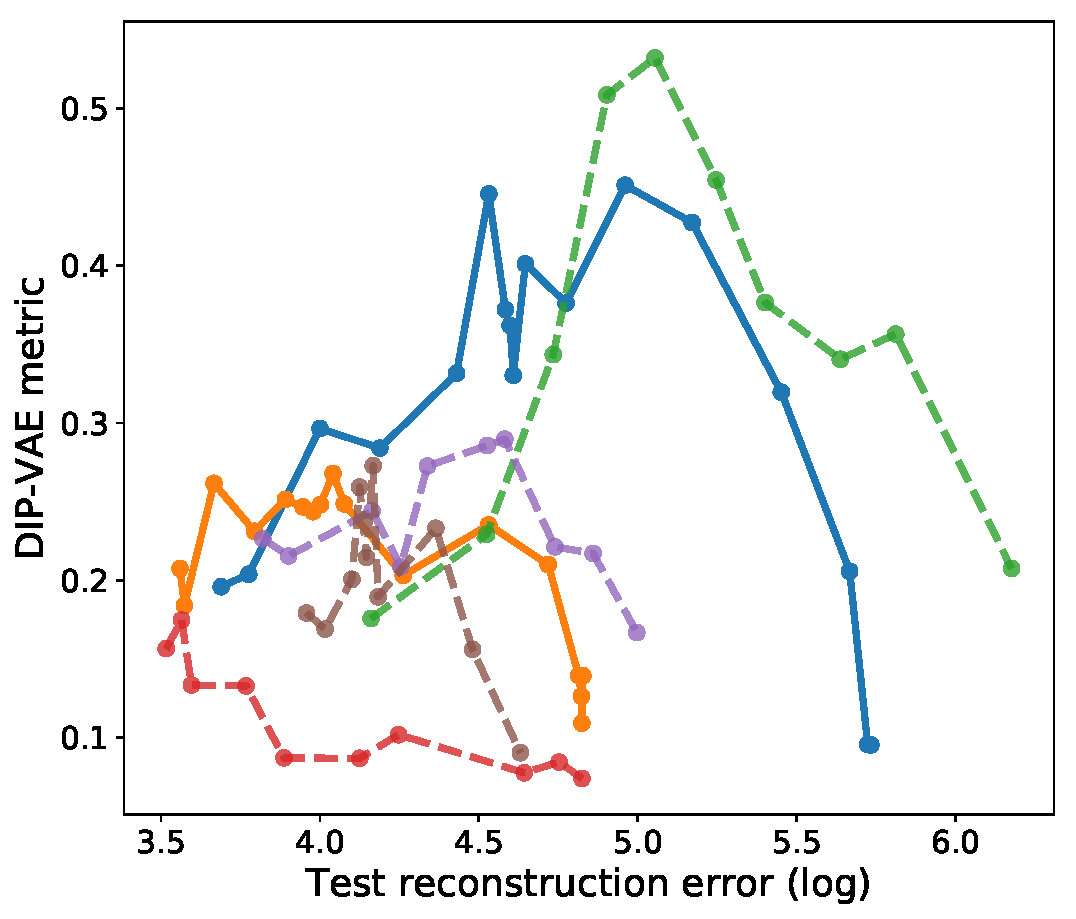
\includegraphics[width=\columnwidth]{figures/subset_DIP_VAE_5_avg_b}
		\caption{}
	\end{subfigure}%
	~ 
	\begin{subfigure}[t]{0.33\textwidth}
	\centering
	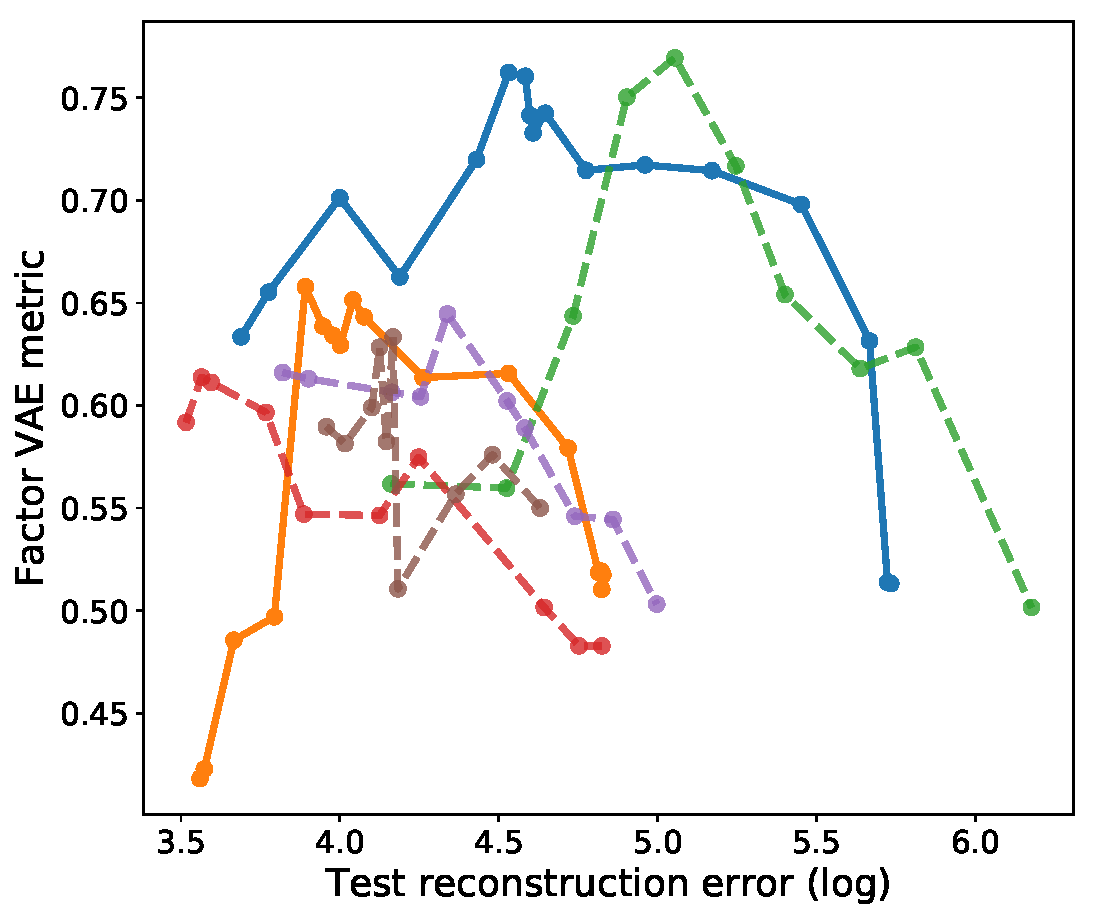
\includegraphics[width=\columnwidth]{figures/subset_factor_VAE_5_avg_b}
	\caption{}
	\end{subfigure}
	\caption{\label{fig:dsprites_disentanglement_partial}Test reconstruction error against disentanglement metrics of {\bf (a)} \cite{HM+17}, {\bf (b)} \cite{kumar2017variational} and {\bf (c)} \cite{kim2018disentangling}. Solid lines are WAE models, dashed lines are baselines. Each line shows how test reconstruction and metric scores vary as the single hyper-parameter for each model was varied (averages over 10 random seeds for each hyper-parameter setting were taken). \textbf{In all plots, up-and-left is better}. WAEs are competitive against all other methods. For Gaussian WAE, $\lambda_1=2.5$ attained the highest disentanglement under all metrics. \label{fig:latent_traversals}}
\end{figure}
%
\paragraph{Quantitative Experiments} We evaluated the performance of probabilistic-encoder WAEs on the disentanglement task as measured by each of the three metrics. 
WAEs are flexible models for which it is possible to specify any encoding distribution and prior, as long as it is possible to sample from them. We considered two configurations, one with a Gaussian prior and encoder, the other with a uniform prior and encoder.
As baselines we also evaluated the performances of the $\beta$-VAE, DIP-VAE, and FactorVAE. The results are summarised in Figure \ref{fig:dsprites_disentanglement_partial}. We describe our experimental procedure here in brief; see Supplementary Materials \ref{appendix:disentanglement} for further details and results.

For all models we used the same fixed fully-connected architecture used by \cite{HM+17} with a Bernoulli (cross-entropy) reconstruction loss and 10 latent dimensions.
All models considered have one tunable hyper-parameter\footnote{For WAE models we kept the weighting of the MMD term $\lambda=400$ fixed and varied only the weighting of the $L_1$ regularisation $\lambda_1$} corresponding to the weighting of the additional regulariser. For several settings of each hyper-parameter, we trained 10 models with different random seeds.
After training, we calculated the average test reconstruction error and score for each metric over these 10 runs. These averages were then plotted in Figure \ref{fig:dsprites_disentanglement_partial}  (so one point in each plot corresponds to one hyper-parameter setting for one model, averaged over 10 random seeds).

The two WAE models were competitive with all other methods, able to achieve a good trade-off between test reconstruction error and disentanglement under all three metrics. In particular, the WAE with Gaussian encoder and prior performed well.

\vspace{-0.2cm}

\paragraph{Qualitative experiments}

We ran probabilistic encoder WAEs on other datasets for which no ground truth generative factors are available. 
In such cases, no metric exists to evaluate disentanglement so this is instead commonly done by inspecting \emph{latent traversals}. Such figures are generated by sampling a point from the latent space and then showing how the output of the decoder changes as we vary the individual coordinates of the latent code. Figure \ref{fig:latent_traversals} shows latent traversals demonstrating learned factors when training on MNIST, 3D Chairs and dSprites.

\begin{figure}
	\begin{minipage}{0.5\textwidth}
		\centering
		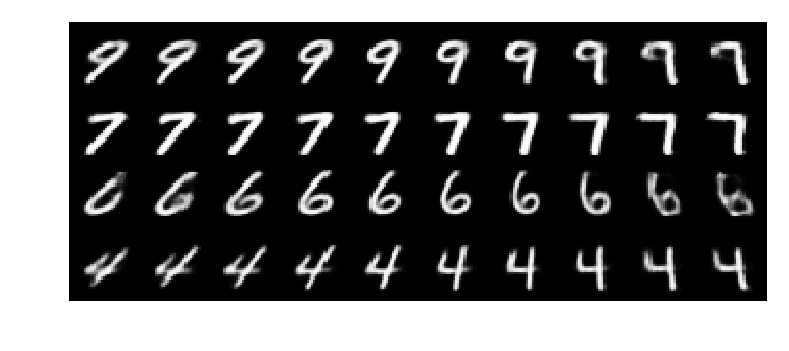
\includegraphics[width=\textwidth]{figures/mnist_slant}
	\end{minipage}%
	\begin{minipage}{0.5\textwidth}
		\centering
		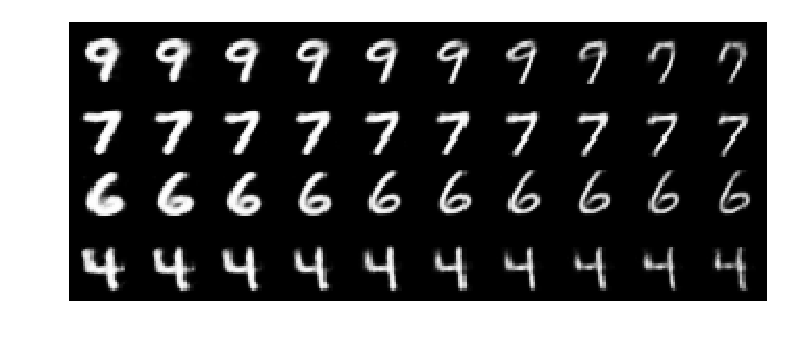
\includegraphics[width=\textwidth]{figures/mnist_thickness}
\end{minipage}

	\begin{minipage}{0.333\textwidth}
		\centering
		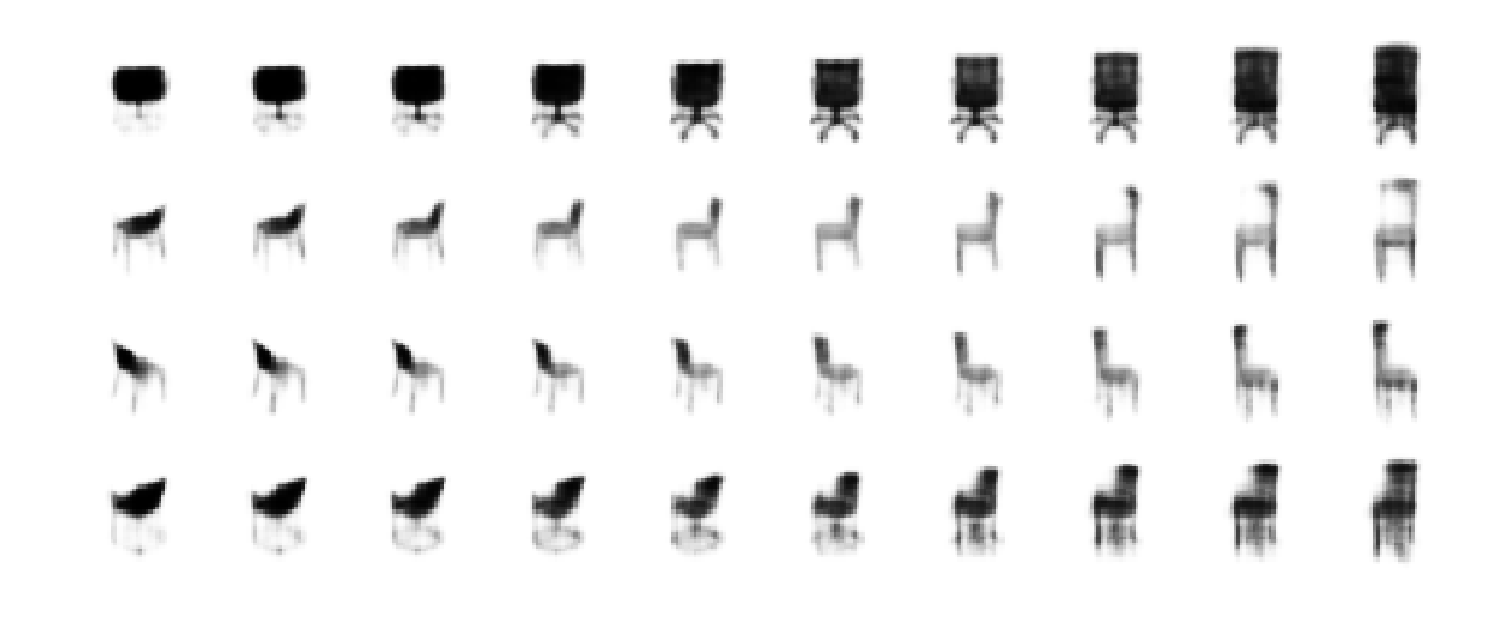
\includegraphics[width=\textwidth]{figures/chairs_back}
	\end{minipage}%
	\begin{minipage}{0.333\textwidth}
		\centering
		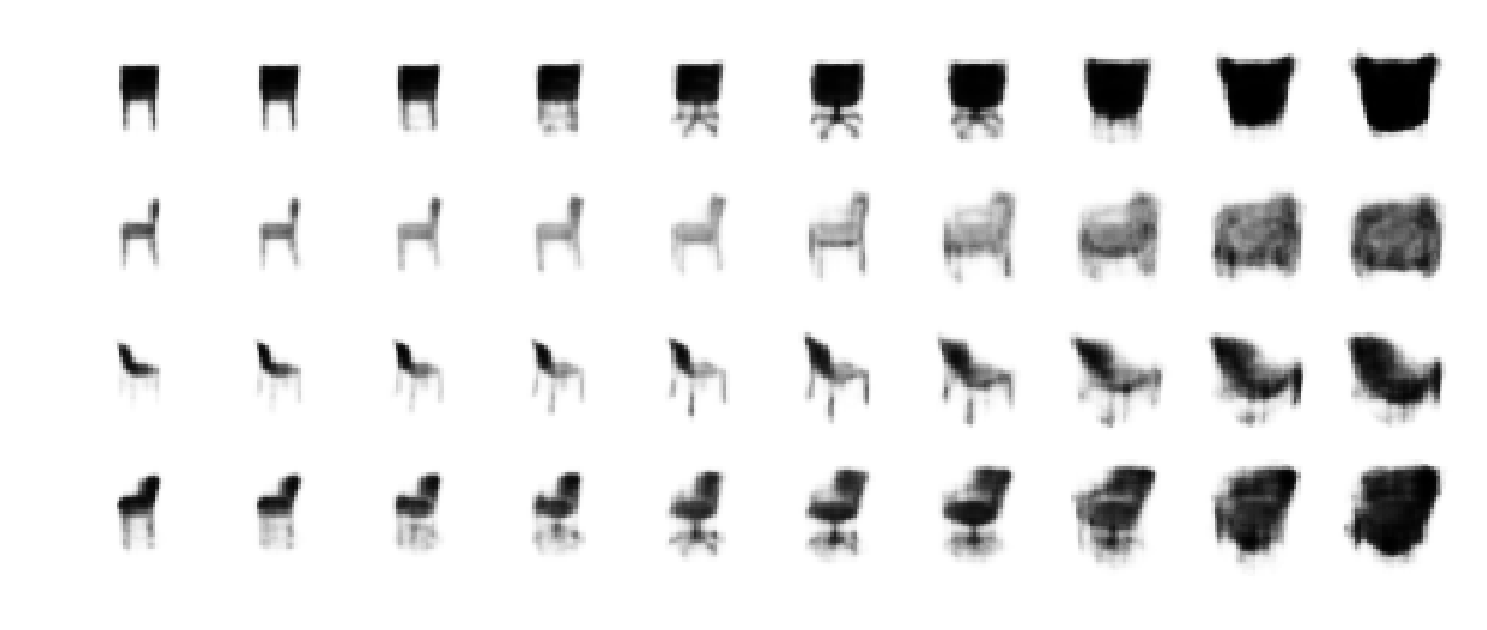
\includegraphics[width=\textwidth]{figures/chairs_size}
	\end{minipage}%
	\begin{minipage}{0.3333\textwidth}
		\centering
		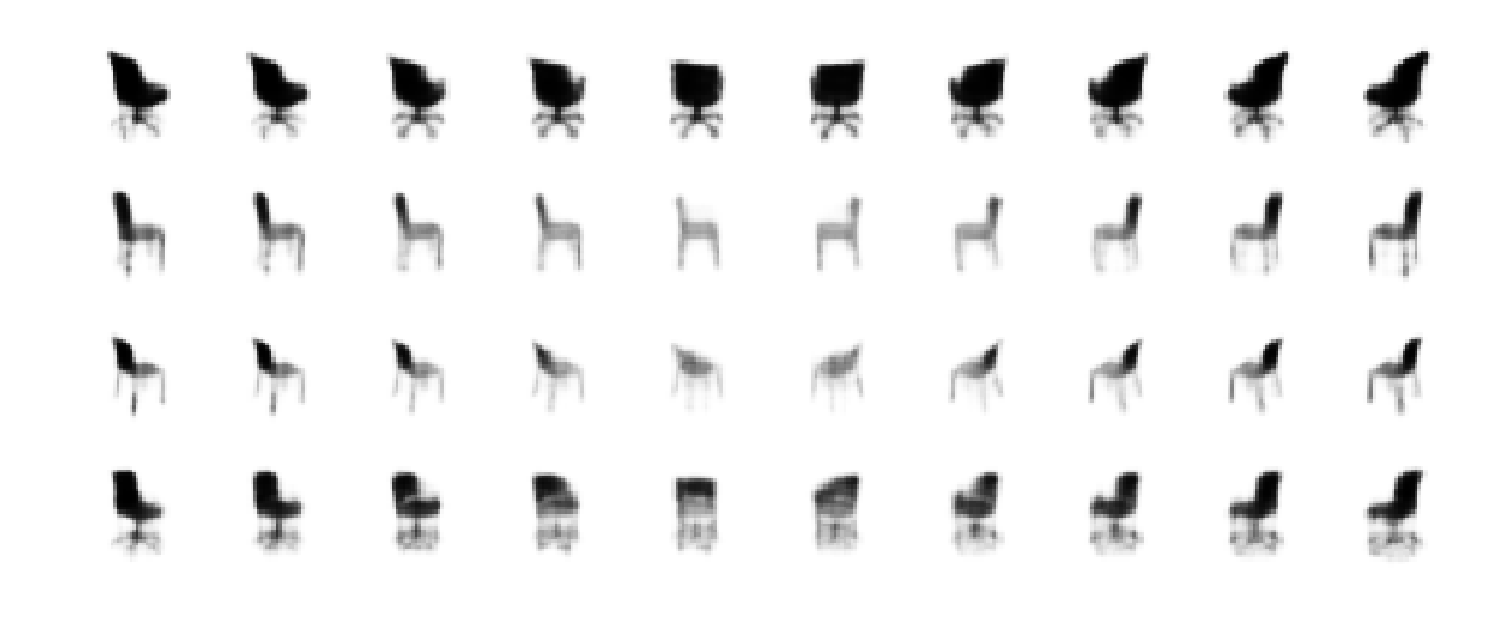
\includegraphics[width=\textwidth]{figures/chairs_azimuth}
	\end{minipage}

	\begin{minipage}{0.333\textwidth}
		\centering
		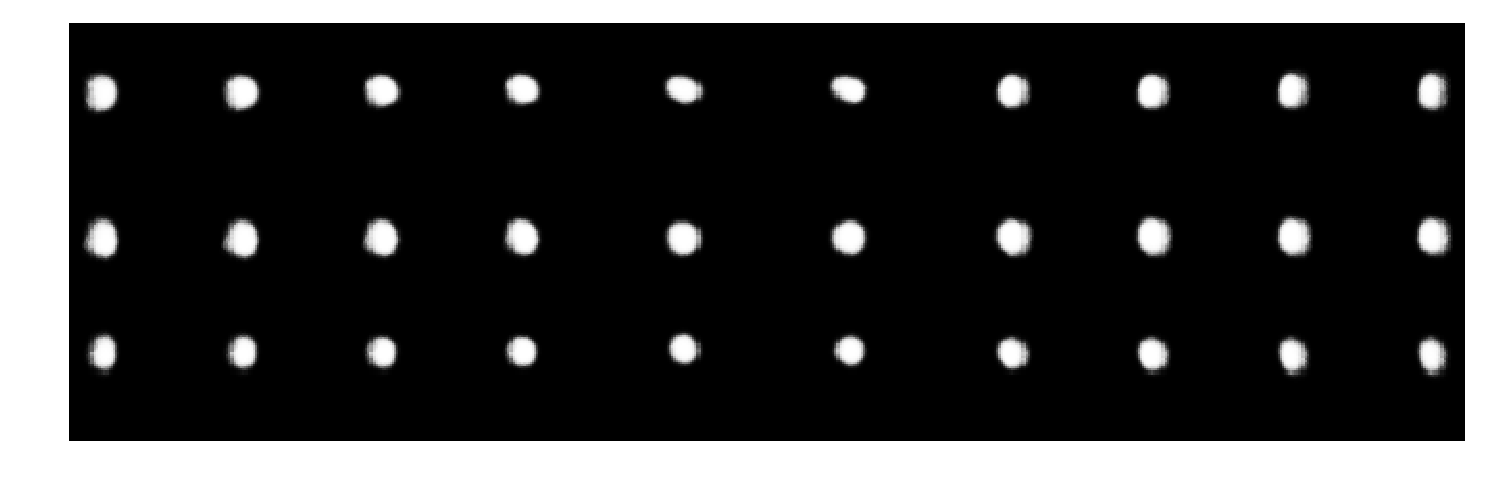
\includegraphics[width=\textwidth]{figures/dsprites_LR}
	\end{minipage}%
	\begin{minipage}{0.333\textwidth}
		\centering
		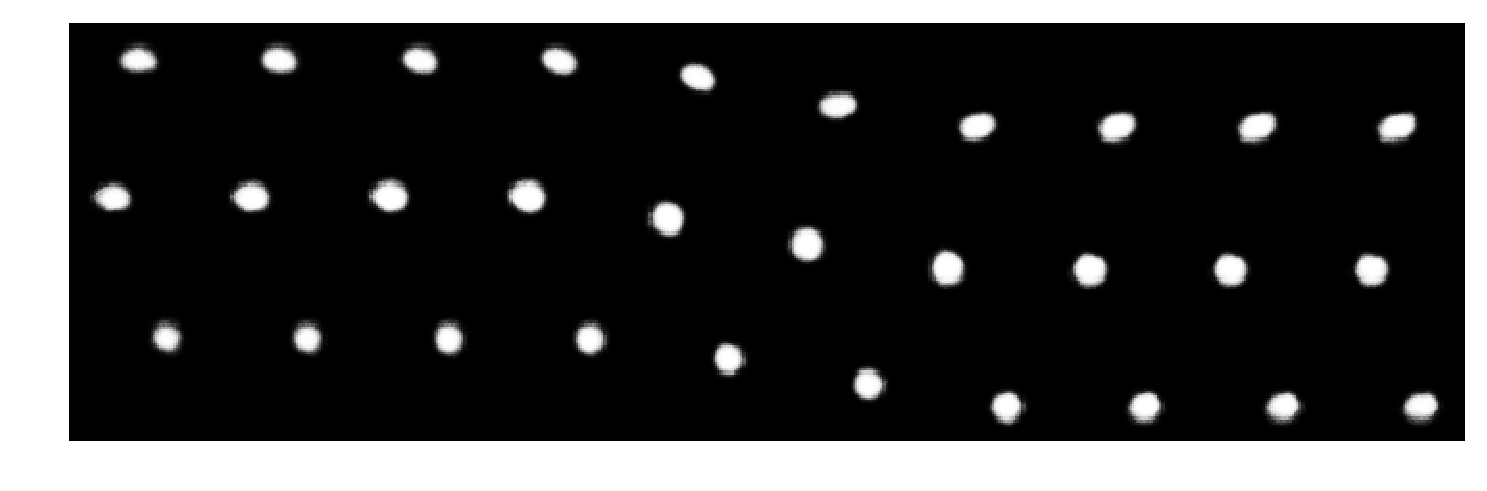
\includegraphics[width=\textwidth]{figures/dsprites_UD}
	\end{minipage}%
	\begin{minipage}{0.3333\textwidth}
		\centering
		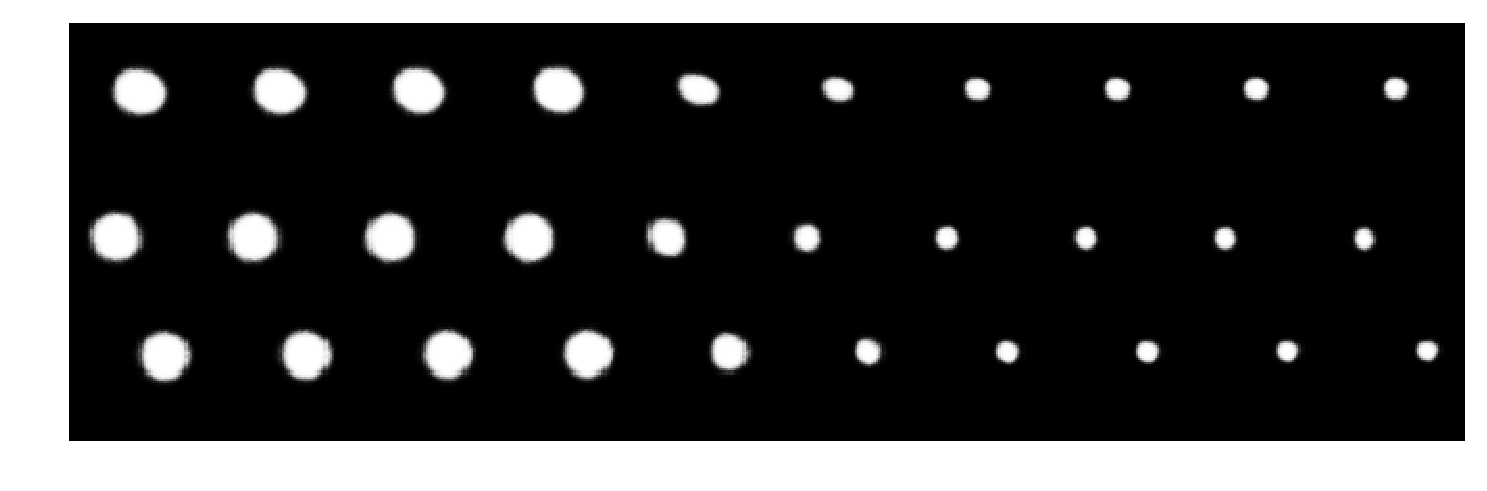
\includegraphics[width=\textwidth]{figures/dsprites_size}
	\end{minipage}
\caption{Various factors in different datasets learned by Gaussian-encoder WAEs. \textbf{Top (MNIST):} slant and thickness ($\lambda_1=1$);
\textbf{Middle (3D Chairs):} Back style, size, azimuth ($\lambda_1=0.5$);  
\textbf{Bottom (dSprites):} X-pos., Y-pos., size ($\lambda_1=2.5$).
Images generated by fixing one code per row and varying one coordinate from left to right within one block of images.
}

\end{figure}

\vspace{-0.2cm}

\section{Conclusion and future directions}

\vspace{-0.2cm}

We investigated the problems that can arise when there is a mismatch between the dimension $\dZ$ of the latent space of a WAE and the intrinsic dimension $\dI$ of the dataset on which it is trained. 
We propose to use probabilistic encoders rather than deterministic encoders to mitigate these problems.
In practice, we found that when probabilistic encoders are used, the original WAE-MMD formulation fails to train properly but that this can be resolved with additional regularisation on the variances of the encoding distributions.
With this regularisation, probabilistic-encoder WAEs are able to adapt to larger latent dimensions.
We applied regularised probabilistic-encoder WAEs to a benchmark disentangled representation learning task on which WAEs performed competitively against state-of-the-art baselines.

One direction for future research is to investigate whether it is possible for probabilistic-encoder WAEs to automatically adapt to $\dZ$ without any hyper-parameter tuning. 
Approaches to this include deriving theoretically justified regularisation to prevent variance collapse and considering other divergence measures that take into account the encoding distribution variances.
The results of our experiments on the disentanglement benchmark combined with the flexibility of the WAE framework indicate that WAEs have the potential to learn useful semantically meaningful representations of data.

%\bibliography{wae18nips}
%\bibliographystyle{abbrvnat}
%
%\newpage 
%\renewcommand\thesection{\Alph{section}}
%\setcounter{section}{0}

\section*{Supplementary Materials}

\section{Details for Fading Squares experiment}\label{appendix:fading_squares}

\subsection{Experimental details}

We trained WAEs with deterministic and random encoders. The architectures we used were:

\textbf{Deterministic encoder:} Input $\mathbb{R}^{32 \times 32}$ $\rightarrow$ FC 1200 units, ReLU $\rightarrow$ FC 1200 units, ReLU $\rightarrow$ FC $\mathbb{R}^2$

\textbf{Probabilistic encoder:} Input $\mathbb{R}^{32 \times 32}$ $\rightarrow$ FC 1200 units, ReLU $\rightarrow$ FC 1200 units, ReLU $\rightarrow$ FC $\mathbb{R}^{2\times 2}$

\textbf{Decoder:} $\mathbb{R}^{2}$ $\rightarrow$ FC 1200 units, tanh $\rightarrow$ FC 1200 units, tanh $\rightarrow$  FC 1200 units, tanh $\rightarrow$  FC $\mathbb{R}^{32\times 32}$

The probabilistic encoder outputs the mean $\mu(X)$ and \emph{log-side-lengths} $\log(\ell(X))$ of an axis aligned box. This parametrises a uniform distribution over an axis aligned box 
%
\begin{align*}
Q(Z|X) = \text{Unif}\left(\prod_{i} [\mu_i(X) - \ell_i(X), \mu_i(X) + \ell_i(X)]\right)
\end{align*}
%
We use the reparametrisation trick to allow back-propagation through sampling $z_n \sim Q(Z| x_n)$
%
\begin{align*}
	\epsilon &\sim \text{Unif}\left([-1, 1]^{\dZ} \right) \\
	z_n &= \mu(x_n)  + \epsilon \odot \ell(X)
\end{align*}
%
where $\odot$ is the element-wise product of two vectors.

Models were trained with the vanilla WAE-MMD Algorithm 2 of \cite{TBG+17}, with $\lambda = 50$, Bernoulli loss and batch size 100. We used the Adam optimizer with learning rate $10^{-3}$ for 40,000 iterations.

\subsection{Preliminary results: implications for WAE-GAN}\label{appendix:wae_gan}

	Preliminary experimentation suggests that the better quality of samples from the {WAE-GAN} compared to the {WAE-MMD} reported in \cite{TBG+17} could be a result of the instability of the associated adversarial training. We found that when training a deterministic-encoder {WAE-GAN} on the \emph{fading squares} dataset, the {1-D} embedding of the data-manifold (the support of $Q_Z$) would move constantly through the support of $P_Z$ throughout training without converging. This means that the decoder is trained on a much larger fraction of the total volume of $P_Z$ compared to the {WAE-MMD}, for which the stability of training means that convergence to the final manifold (constituting a small fraction of $P_Z$) is quick.


\subsection{Incorrect proportions of generated images}\label{appendix:wrong_proportions}

To see that the decoded images were generated in incorrect proportions, consider the mean pixel value of an image in the toy \emph{fading squares} dataset. It is a 1-dimensional random variable, uniformly distributed on the interval $[0, 36/1024]$, where $36/1024$ is the mean (over the whole image) in the case of a white square. We trained $5$ deterministic- and probabilistic-encoder WAEs, and for each one estimated the cumulative distribution function (CDF) of the mean pixel values with 100,000 sampled images.
As a baseline, we also ran this procedure using $5$ VAEs with the same architecture.

This is summarised in Figure \ref{fig:fading-squares-deviation-from-cumulative}, which displays the deviation from the theoretical CDF for each of the models trained. This shows that the deviation from the theoretical distribution for deterministic-encoder WAEs is consistently worse than for the probabilistic-encoder WAEs and VAEs, which fair comparably with one another. Note that while observing a uniform distribution here does not prove that images are generated with the correct frequencies, deviation from it does indeed indicate failure.

\begin{figure}[t!]
	\centering
	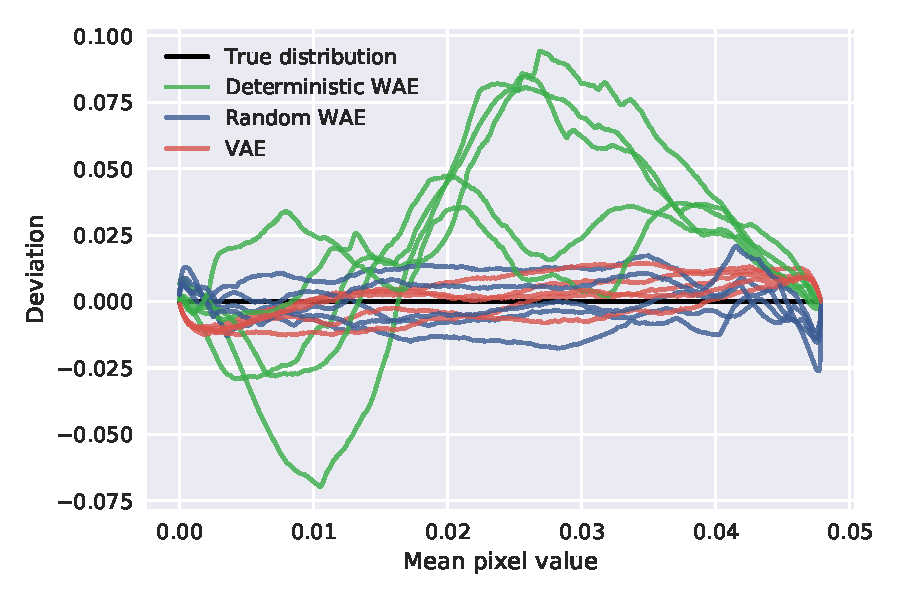
\includegraphics[width=0.5\columnwidth]{figures/fading-square-deviation-from-true-cumulative-distribution}
	\caption{\label{fig:fading-squares-deviation-from-cumulative} Deviation from the correct cumulative distribution of the mean pixel values for models trained on the \emph{fading squares} dataset. If images were generated using the correct frequencies, the deviations should be close to $0$. The deterministic WAE does not meet this goal.}
\end{figure}



\section{Details for CelebA experiments}\label{appendix:celebA}

We preprocessed the CelebA dataset by centre-cropping and down-sampling so that all images are $64\times 64$ pixels. 
In all experiments ran using the CelebA dataset (i.e. those summarised in Table \ref{table:dimension-fid-test-reconstruction} and Figure \ref{fid:celebA-fid-test-errors-vs-latent-dim}) we used  DC-GAN architectures with $3$ layers, $4\times 4$ kernels and up to $128$ filters. Specifically:

\textbf{Deterministic Encoders:} Input $\mathbb{R}^{64 \times 64 \times 3}$ $\rightarrow$ $4\times 4$ convolution 32 filters, stride 2, batch norm, ReLU $\rightarrow$ $4\times 4$ convolution 64 filters, stride 2, batch norm, ReLU $\rightarrow$ $4\times 4$ convolution 128 filters, stride 2 $\rightarrow$ FC $\mathbb{R}^{\dZ}$

\textbf{Probabilistic Encoders:} Input $\mathbb{R}^{64 \times 64 \times 3}$ $\rightarrow$ $4\times 4$ convolution 32 filters, stride 2, batch norm, ReLU $\rightarrow$ $4\times 4$ convolution 64 filters, stride 2, batch norm, ReLU $\rightarrow$ $4\times 4$ convolution 128 filters, stride 2 $\rightarrow$ FC $\mathbb{R}^{\dZ \times 2}$

\textbf{Decoders:} Input $\mathbb{R}^{\dZ}$ $\rightarrow$ FC $8 \times 8 \times 128$ ReLU $\rightarrow$ transposed convolution, 64 filters, stride 2, batch norm, ReLU $\rightarrow$ transposed convolution, 32 filters, stride 2, batch norm, ReLU $\rightarrow$ transposed convolution, 3 filters, stride 2.

We used Gaussian encoders for all probabilistic encoders. The same as in a standard VAE, we used the encoder to parametrise the mean $\mu(X)$ and log-variances $\log(\Sigma(X))$ of a diagonal-constrained Gaussian. We use the reparametrisation trick to back-propagate through sampling $z \sim \mathcal{N}\left(\mu(X), \Sigma(X)\right)$

\begin{align*}
	\epsilon &\sim \mathcal{N}\left(0, I\right)\\
	z &= \mu(X) + \epsilon \odot \exp\left( \log\Sigma(X) / 2\right)
\end{align*}

Models were trained with the vanilla WAE-MMD Algorithm 2 of \cite{TBG+17}, with the objective function modified with the addition of our new $L_1$ regulariser in the case of the probabilistic encoders. Additionally, we found that with little or no $L_1$ regularisation, the log-variances of the probabilistic encoders would become very negative and would cause numerical issues when back-propagating. To avoid these problems we clipped the log-variances to be no less than $-20$.

In all cases we used $\lambda = 400$, Bernoulli reconstruction loss and batch size 100. We used the Adam optimizer with learning rate $10^{-4}$ for 16 epochs, then $10^{-5}$ for a further 16 epochs (hence 32 epochs in total).

For the experiments to make Figure \ref{fid:celebA-fid-test-errors-vs-latent-dim} we used $\lambda_1 \in \{0, 1\!\times\!10^{-3},  3\!\times\! 10^{-3}, 1\!\times\! 10^{-2}, 3\!\times\! 10^{-2}, 1\!\times\! 10^{-1}, 3\!\times\! 10^{-1}, 1, 3\}$



\section{Details for disentanglement experiments}\label{appendix:disentanglement}

For all experiments in the disentanglement section (Figures \ref{fig:dsprites_disentanglement_partial} and \ref{fig:latent_traversals}), we used the same architecture as proposed by \cite{HM+17} with latent dimension $\dZ=10$ and Bernoulli loss.

\textbf{Encoder:} Input $\mathbb{R}^{64 \times 64}$ $\rightarrow$ FC 1200 units, ReLU $\rightarrow$ FC 1200 units, ReLU $\rightarrow$ FC $\mathbb{R}^{10\times 2}$

\textbf{Decoder:} $\mathbb{R}^{10}$ $\rightarrow$ FC 1200 units, tanh $\rightarrow$ FC 1200 units, tanh $\rightarrow$  FC 1200 units, tanh $\rightarrow$  FC $\mathbb{R}^{64\times 64}$

We downsampled the 3D Chairs images to $64\!\times\!64$ pixels. We padded the MNIST images to make them $32\!\times\!32$ pixels. For MNIST, we used the same architectures but with $32\!\times\!32$ inputs and outputs for the encoder and decoders respectively.

\subsection{WAE specific details}

On the dSprites task, we tested four different types of WAE.

\textbf{WAE Uniform:} We used a uniform prior over the box $[-1, 1]^{\dZ}$ and parametrised the uniform distribution over an axis-aligned box with the encoder, using the reparametrisation trick as described in Appendix \ref{appendix:fading_squares}. Additionally we constrained the mean $\mu(X)$ to be within the set $[-1,1]^{\dZ}$ by adding a tanh activation.

\textbf{WAE Gaussian:} We used a Gaussian prior and parametrised a diagonally-constrained Gaussian with the encoder, using the reparametrisation trick as described in Appendix \ref{appendix:celebA}. Additionally we constrained the mean $\mu(X)$ to be within the set $[-1,1]^{\dZ}$ by adding a tanh activation.

Results from the above two models were presented in Figure \ref{fig:dsprites_disentanglement_partial}. We additionally tested the following two models, which are the same except we do not constrain the means to be within the set $[-1,1]^{\dZ}$.

\textbf{WAE Uniform (no tanh):} We used a uniform prior over the box $[-1, 1]^{\dZ}$ and parametrised the uniform distribution over an axis-aligned box with the encoder, using the reparametrisation trick as described in Appendix \ref{appendix:fading_squares}.

\textbf{WAE Gaussian (no tanh):} We used a Gaussian prior and parametrised a diagonally-constrained Gaussian with the encoder, using the reparametrisation trick as described in Appendix \ref{appendix:celebA}. 

For each WAE model, we fixed $\lambda=400$ and varied $\lambda_1$. For each value of $\lambda_1$, we trained 10 models with different random seeds. All models were trained with batch size 100 with the Adam Optimiser for 30,000 iterations with learning rate $10^{-3}$ and a further 30,000 iterations with learning rate $10^{-4}$.

For each of these 10 models per hyper-parameter setting we calculated each of the disentanglement metrics as well as the test reconstruction, and took their average. For the $\beta$-VAE metric which involves stochastically training a classifier, we evaluated the metric three times and took the maximum to be the value of the metric. 

For all WAE models we searched over $\lambda_1 \in \{0, 0.1, 0.5, 1, 2, 2.5, 2.8, 3, 3.2, 3.5, 5, 8, 12, 18, 25, 40, 60\}$ 

\subsection{Baseline specific details}

Open source implementations were not available for FactorVAE, DIP-VAE-I or DIP-VAE-II, so we implemented these models ourselves based on the detailed descriptions given in \cite{kim2018disentangling} and \cite{kumar2017variational}. \textbf{Our implementations will be open sourced upon publication of this work.}

\textbf{FactorVAE:} It should be noted that the evaluations performed by \cite{kim2018disentangling} use a different architecture to that used in this paper (we use the same architectures used in \cite{HM+17} and \cite{kumar2017variational}) and hence the disentanglement scores we obtain in this work are different to those reported by the authors themselves.

FactorVAE has a single hyper-parameter $\gamma$ which is the weighting of the regulariser they introduce additional to the original VAE objective. We searched over $\gamma \in \{1, 5, 10, 20, 35, 50, 100, 200, 500, 1000\}$. 

The additional regulariser of FactorVAE is adversarially estimated, and thus training involves alternating steps to optimise the auto-encoder and the adversary. We trained with batch size 100 and the Adam Optimiser for both the auto-encoder and the adversary.  We trained for 30,000 iterations with learning rates $10^{-3}$ and $10^{-4}$ for the auto-encoder and adversary respectively, then a further 30,000 iterations with learning rates $10^{-4}$ and $10^{-5}$.

\textbf{DIP-VAE:} The two versions of DIP-VAE involve adding an additional regulariser to the VAE objective. For both versions there are two hyper-parameters $\lambda_d$ and $\lambda_{od}$ (weightings of `diagonal' and `off-diagonal' terms in the regulariser). \cite{kumar2017variational} propose that for DIP-VAE-i one should set $\lambda_d = 10\lambda_{od}$ and for DIP-VAE-ii $\lambda_d = \lambda_{od}$ for the dSprites dataset. 
For both DIP-VAE-i and DIP-VAE-ii we  searched over ${\lambda_{od} \in \{1, 2, 5, 10, 20, 50, 100, 500, 1000, 2000\}}$. We trained with batch size 100 and Adam Optimiser with learning rate $10^{-3}$ for 30,000 iterations and $10^{-4}$ for a further 30,000 iterations.

\textbf{$\beta$-VAE:} We searched over $\beta \in \{1, 3, 10, 20, 30, 40, 50, 75, 100, 150, 200, 300\}$.

\subsection{A note on the disentanglement metrics}
Open source implementations were not available for any of the disentanglement metrics, so we implemented them ourselves based on the detailed descriptions given in the papers. \textbf{Our implementations will be open sourced upon publication of this work.} 


\subsection{Additional results}

In Figure \ref{fig:all_disentanglement} we summarise the disentanglement scores for all models considered.

In particular, observe that the WAE models \emph{without} the tanh-constrained means perform rather poorly. For the Uniform WAE, this may be because the tanh makes training easier by constraining the mean to land where the prior has support. It is curious, however, that tanh-constraint improves the performance of Gaussian WAE. We suspect this is because constraining the means to lie in the interval $[-1, 1]$ forces the model to have non-zero variances in order to put probability mass outside of this interval where $P_Z$ has support.

\begin{figure}
	\begin{minipage}{0.5\columnwidth}
	\begin{center}
		\textbf{Our methods}
	\end{center}
\end{minipage}%
\begin{minipage}{0.5\columnwidth}
	\begin{center}
		\textbf{Baselines}
	\end{center}
\end{minipage}
\begin{minipage}{0.5\columnwidth}	
	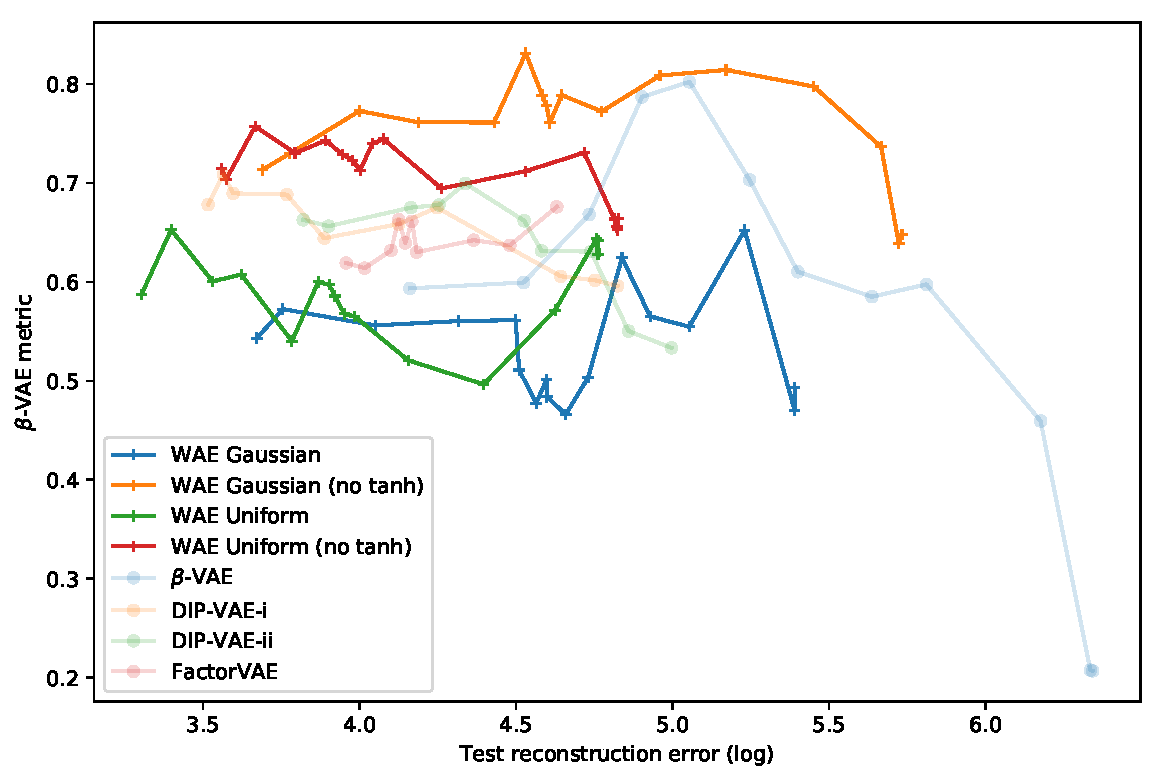
\includegraphics[width=\columnwidth]{figures/beta_VAE_5_avg_b}
	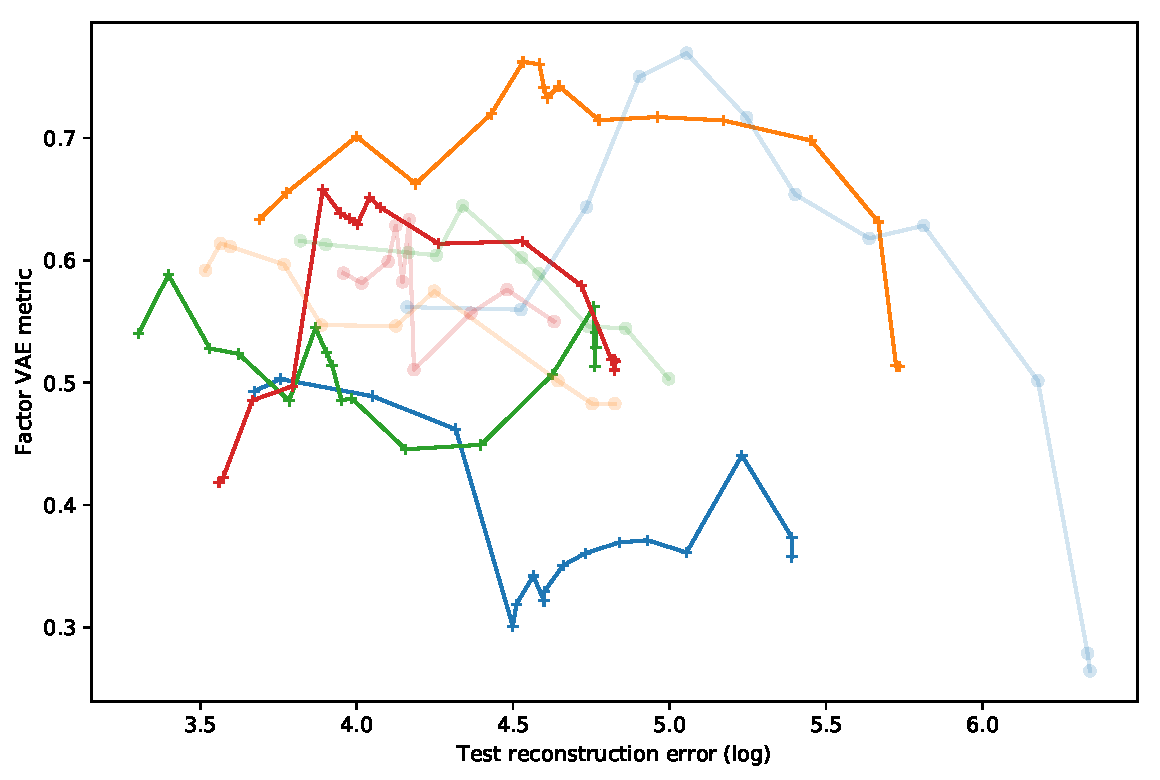
\includegraphics[width=\columnwidth]{figures/factor_VAE_5_avg_b}
	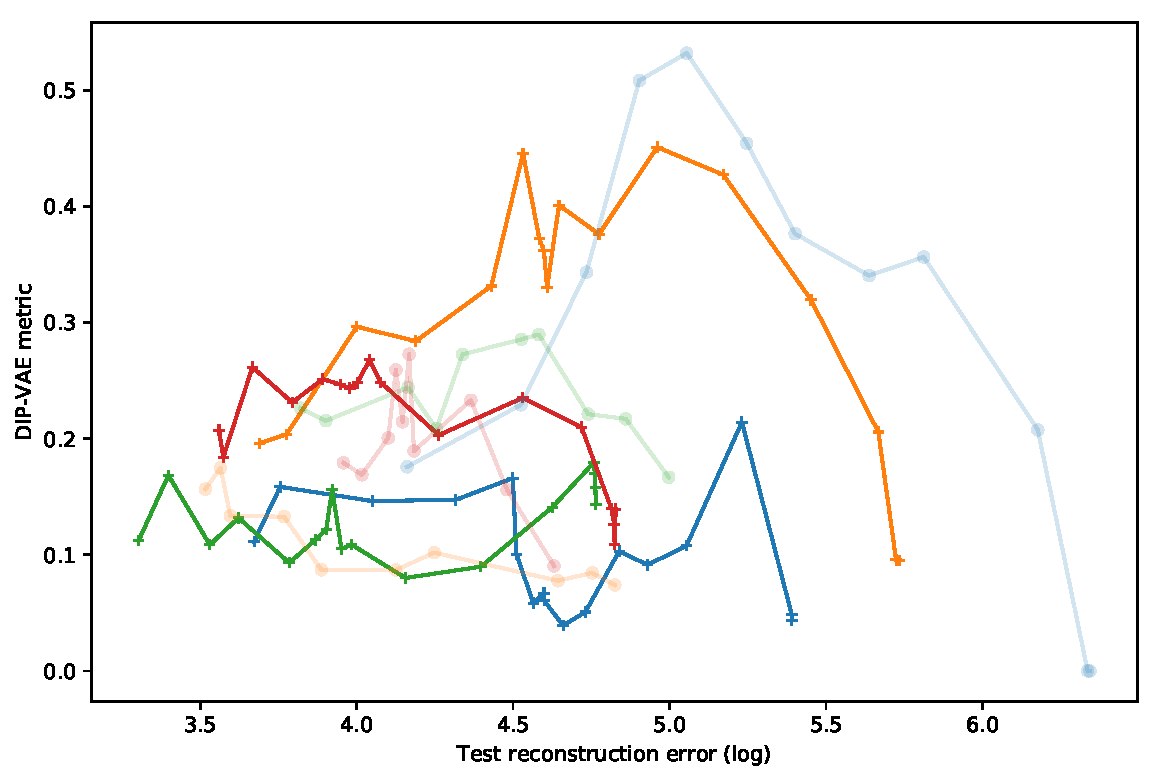
\includegraphics[width=\columnwidth]{figures/DIP_VAE_5_avg_b}
\end{minipage}%
\begin{minipage}{0.5\columnwidth}
	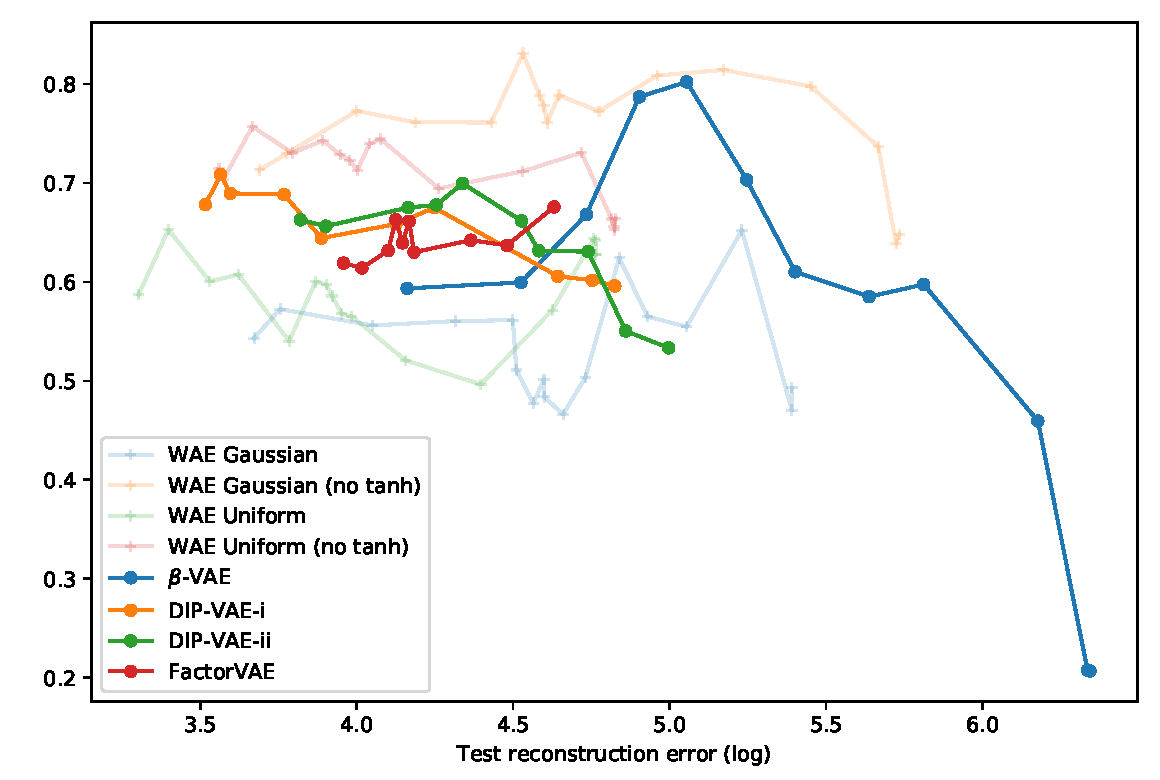
\includegraphics[width=\columnwidth]{figures/beta_VAE_5_avg_a}
	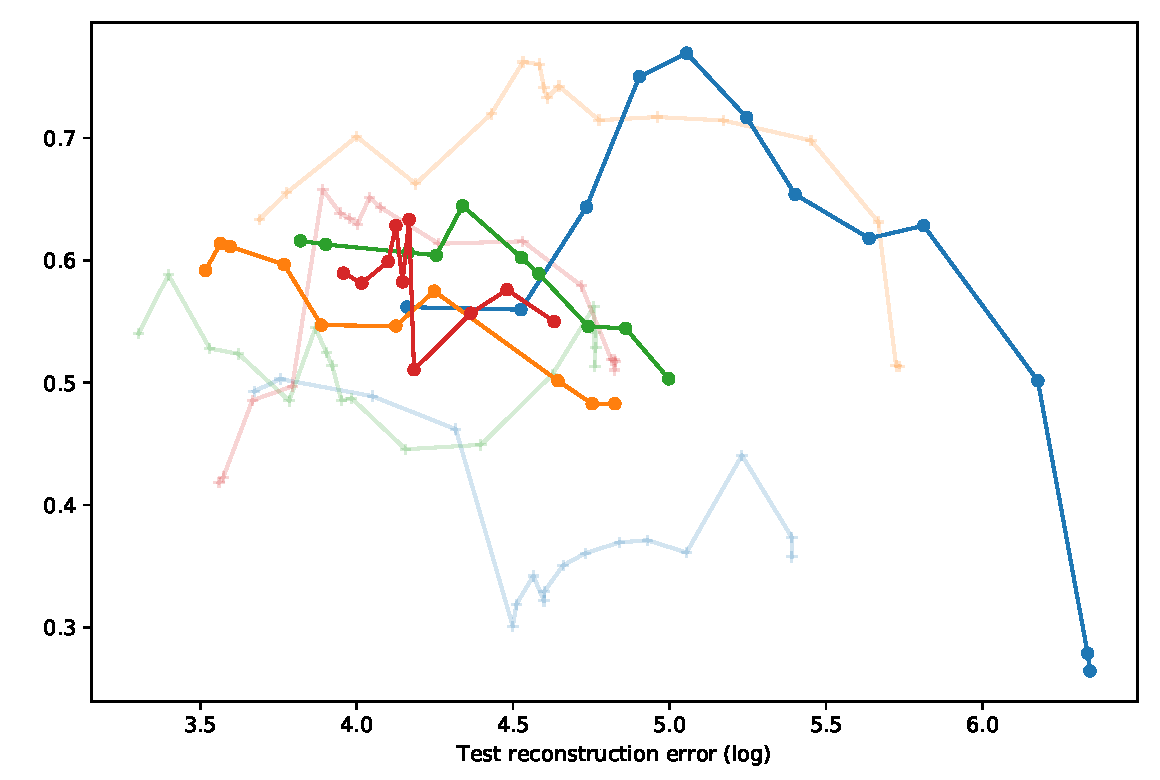
\includegraphics[width=\columnwidth]{figures/factor_VAE_5_avg_a}
	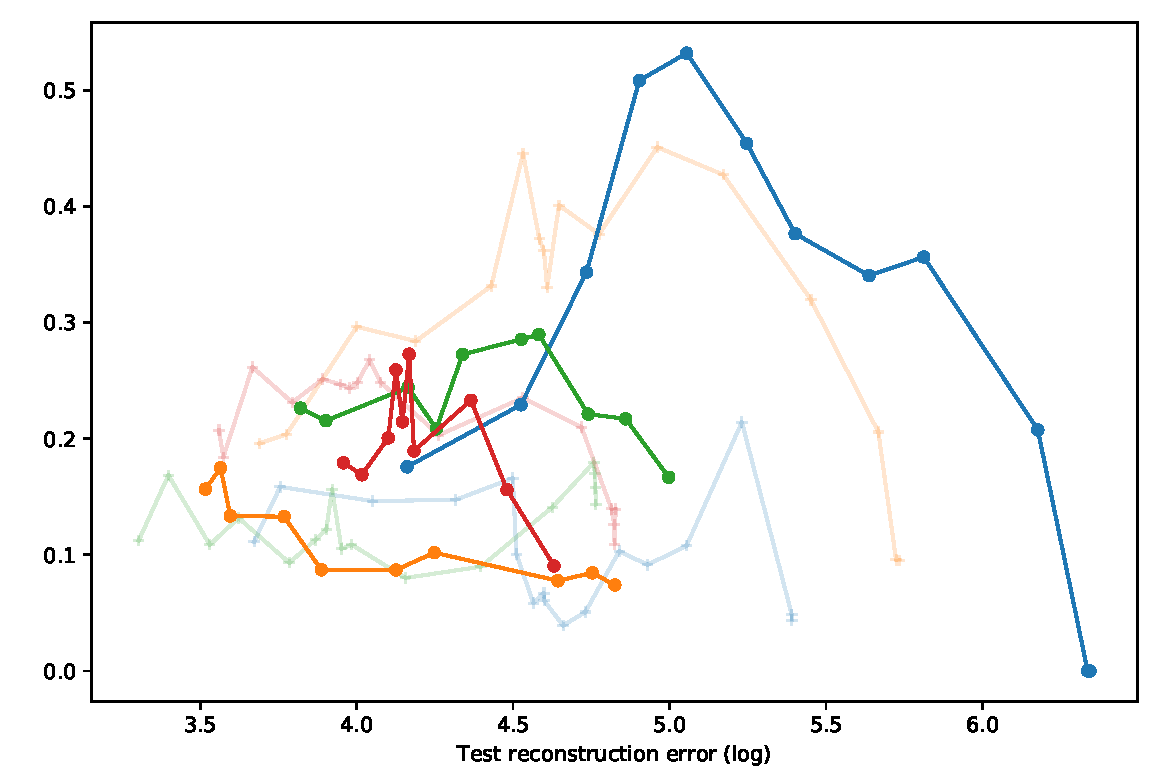
\includegraphics[width=\columnwidth]{figures/DIP_VAE_5_avg_a}	
\end{minipage}
\caption{\label{fig:all_disentanglement} Results of disentanglement metric experiments on all evaluated models.}
\end{figure}


\begin{figure}
	\begin{minipage}{0.5\columnwidth}
		\begin{center}
			\textbf{Our methods}
		\end{center}
	\end{minipage}%
	\begin{minipage}{0.5\columnwidth}
		\begin{center}
			\textbf{Baselines}
		\end{center}
	\end{minipage}
	\begin{minipage}{0.5\columnwidth}	
		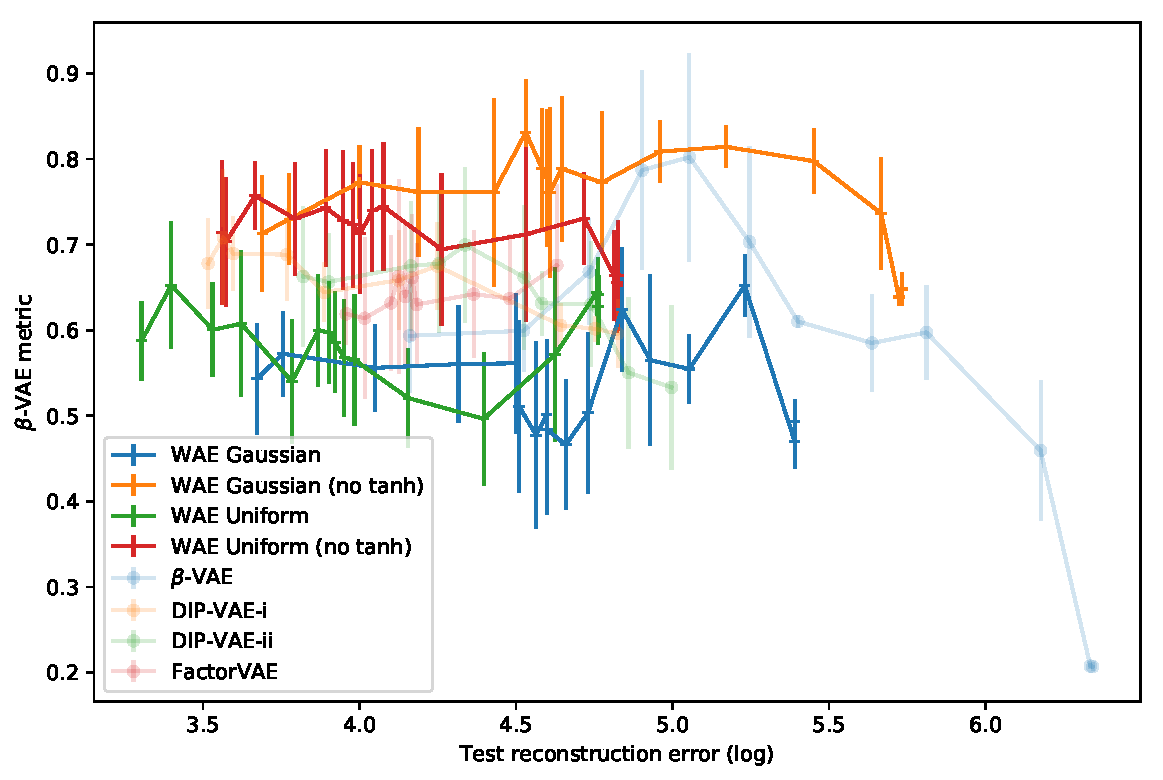
\includegraphics[width=\columnwidth]{figures/error_bars_beta_VAE_5_avg_b}
		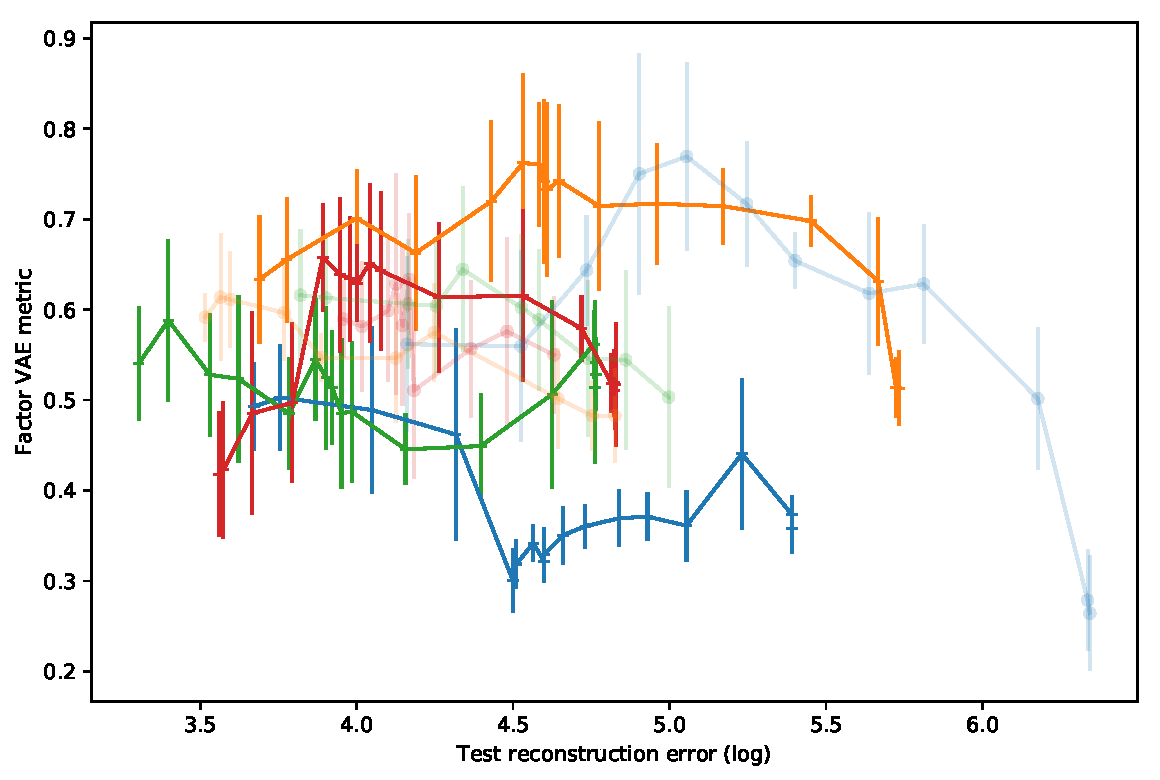
\includegraphics[width=\columnwidth]{figures/error_bars_factor_VAE_5_avg_b}
		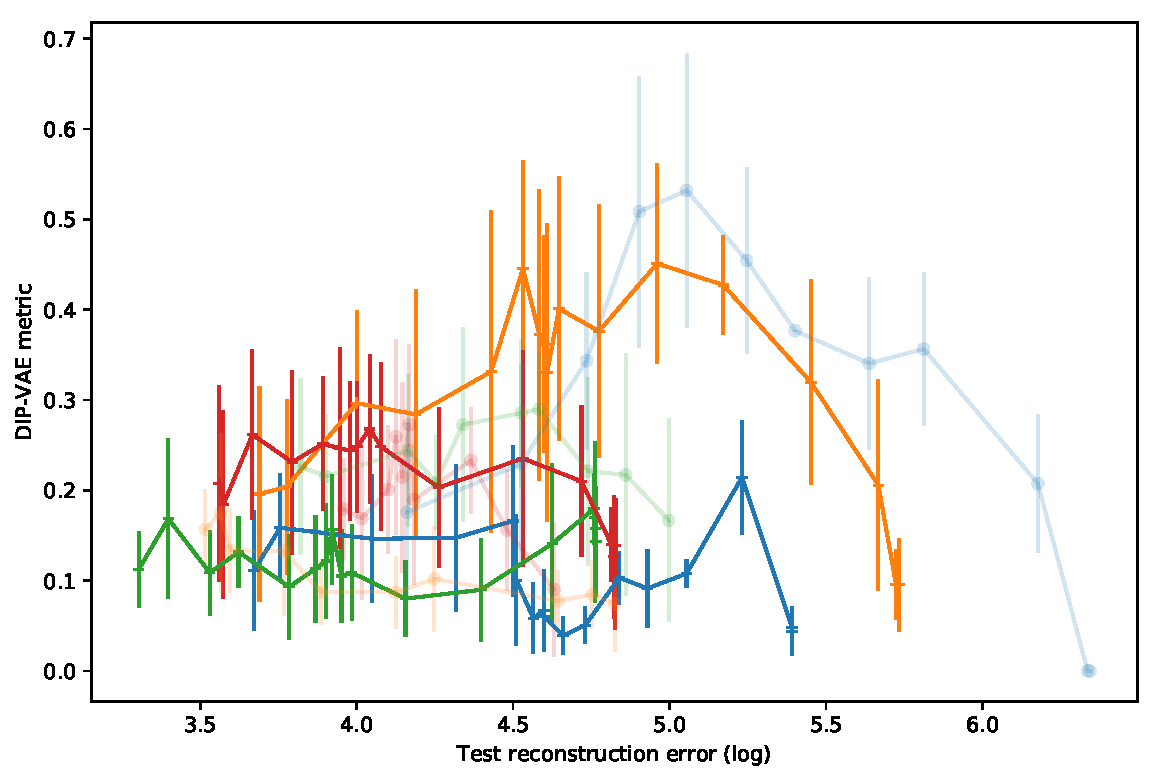
\includegraphics[width=\columnwidth]{figures/error_bars_DIP_VAE_5_avg_b}
	\end{minipage}%
	\begin{minipage}{0.5\columnwidth}
		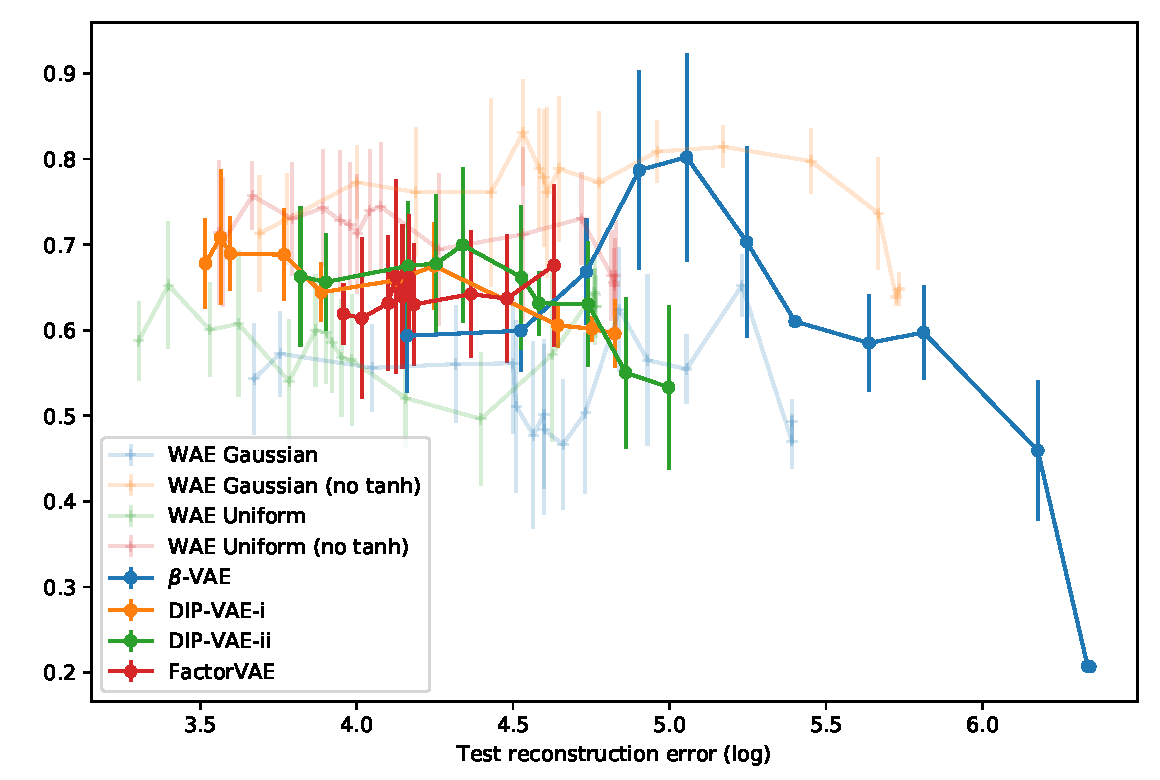
\includegraphics[width=\columnwidth]{figures/error_bars_beta_VAE_5_avg_a}
		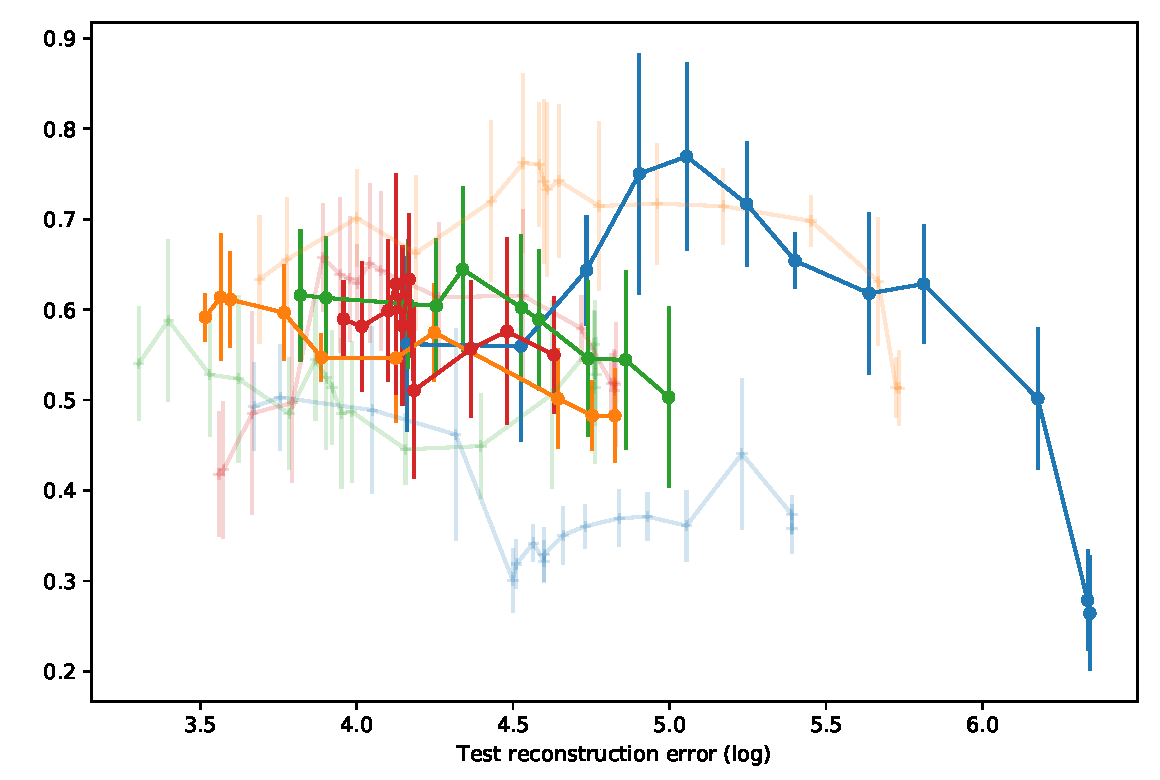
\includegraphics[width=\columnwidth]{figures/error_bars_factor_VAE_5_avg_a}
		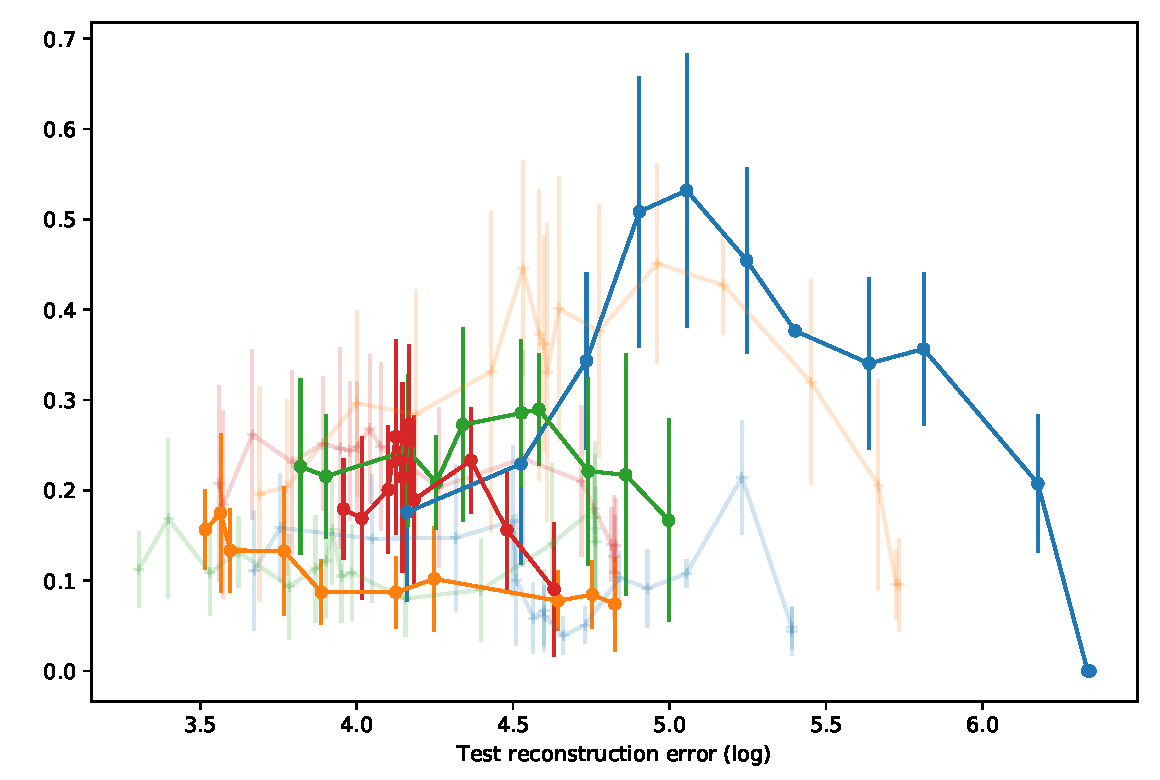
\includegraphics[width=\columnwidth]{figures/error_bars_DIP_VAE_5_avg_a}	
	\end{minipage}
	\caption{\label{fig:all_disentanglement_error_bars} The same as Figure \ref{fig:all_disentanglement} but with error bars showing $\pm$ one standard deviation.}
\end{figure}

